\documentclass[defaultstyle,10pt,master,Helvetica]{./components/thesis}

\usepackage{ucs}
\usepackage[utf8x]{inputenc}
 \usepackage[english]{babel}
\usepackage{amsmath, amsthm, amssymb, amsfonts}
\usepackage{multirow}
\usepackage{colortbl}
\usepackage{ctable}
\usepackage{booktabs}
\usepackage{graphicx}
\usepackage[hang,small,bf]{subfigure}
\usepackage{algorithmic}
\usepackage[chapter]{algorithm}
\usepackage{cite}
\usepackage[printonlyused]{acronym}
\usepackage{./components/extra_functions}
\usepackage{hhline}
\usepackage{tabularx}
\usepackage{hyperref}
\hypersetup{ a4paper=true,
             colorlinks=false,
             citecolor=red,
             breaklinks=true,
             bookmarks=true,
             bookmarksnumbered=true,
             bookmarksopen=true,
             pdftitle={TTSP - Tagus Time Synchronization Protocol},
             pdfauthor={Hugo Miguel Pinho Freire},
             pdfsubject={TTSP - Tagus Time Synchronization Protocol: An Adaptive Approach to Time Synchronization in Tagus-SensorNet}, 
             pdfcreator={Hugo Miguel Pinho Freire},  
             pdfkeywords={Wireless Sensor Networks, Time Synchronization, TTSP} 
}
\usepackage{url} 
\usepackage{acronym}

\renewcommand{\theparagraph}{\Alph{paragraph}~--}
\hoffset 0in
\voffset 0in
\oddsidemargin 2 cm
\evensidemargin 2 cm
\marginparsep 0in
\topmargin -0.25 cm
\textwidth 12.5 cm
\textheight 22.4 cm

% ########################################################
% Fomatting for The Fancy Headers
\usepackage{fancyhdr}
\pagestyle{fancy}
\renewcommand{\chaptermark}[1]{\markboth{\thechapter.\ #1}{}}
\renewcommand{\sectionmark}[1]{\markright{\thesection\ #1}}
% x-x-x-x-x-x-x-x-x-x-x-x-x-x-x-x-x-x-x-x-x-x-x-x-x-x-x-x-x-x-x-x-x-x-x-x-x-x-x-x
% comment next 3 lines if no Header and Hooter on every page
% For IST MSc Thesis do not use Header nor Footer 
%\fancyhf{} \fancyhead[LE]{\bfseries\nouppercase{\leftmark}} % comment for IST MSc Thesis
%\fancyhead[RO]{\bfseries\nouppercase{\rightmark}} % comment for IST MSc Thesis
%\fancyfoot[LE,RO]{\bfseries\thepage} % comment for IST MSc Thesis
% x-x-x-x-x-x-x-x-x-x-x-x-x-x-x-x-x-x-x-x-x-x-x-x-x-x-x-x-x-x-x-x-x-x-x-x-x-x-x-x
\fancyhead{}
\renewcommand{\headrulewidth}{0.0pt}
\renewcommand{\footrulewidth}{0.0pt}
\addtolength{\headheight}{2pt} % make space for the rule
\fancypagestyle{plain}{%
   \fancyhead{} % get rid of headers
   \renewcommand{\headrulewidth}{0pt} % and the line
   \renewcommand{\footrulewidth}{0pt}
}
\fancypagestyle{blank}{%
   \fancyhf{} % get rid of headers and footers
   \renewcommand{\headrulewidth}{0pt} % and the line
   \renewcommand{\footrulewidth}{0pt}
}
\fancypagestyle{abstract}{%
   \fancyhead{}
   \renewcommand{\headrulewidth}{0pt}
   \renewcommand{\footrulewidth}{0.0pt}
}
\fancypagestyle{document}{% 
	% x-x-x-x-x-x-x-x-x-x-x-x-x-x-x-x-x-x-x-x-x-x-x-x-x-x-x-x-x-x-x-x-x-x-x-x-x-x-x-x
	% comment next 3 lines if no Header and Hooter on every page
	% For IST MSc Thesis do not use Header nor Footer
%	\fancyhf{} \fancyhead[LE]{\bfseries\nouppercase{\leftmark}} % comment for IST MSc Thesis
%	\fancyhead[RO]{\bfseries\nouppercase{\rightmark}} % comment for IST MSc Thesis
%	\fancyfoot[LE,RO]{\bfseries\thepage} % comment for IST MSc Thesis
	% x-x-x-x-x-x-x-x-x-x-x-x-x-x-x-x-x-x-x-x-x-x-x-x-x-x-x-x-x-x-x-x-x-x-x-x-x-x-x-x
	\fancyhead{}
	\renewcommand{\headrulewidth}{0.0pt}
	\renewcommand{\footrulewidth}{0.0pt}
	\addtolength{\headheight}{2pt} % make space for the rule
}
\setcounter{secnumdepth} {5}
\setcounter{tocdepth} {5}
\renewcommand{\thesubsubsection}{\thesubsection.\Alph{subsubsection}}

\renewcommand{\subfigtopskip}{0.3 cm}
\renewcommand{\subfigbottomskip}{0.2 cm}
\renewcommand{\subfigcapskip}{0.3 cm}
\renewcommand{\subfigcapmargin}{0.2 cm}


\begin{document}


\pdfbookmark[0]{Titlepage}{Title}

\univlogo{2cm}{2cm}{./images/01-istutl}

\title{TTSP - Tagus Time Synchronization Protocol}
\subtitle{An Adaptive Approach to Time Synchronization in Tagus-SensorNet}
\author{Hugo Miguel Pinho Freire}
\degree{Engenharia de Redes de Comunicações}
\supervisor{Prof. Doutor Rui Manuel Rodrigues Rocha}
\date{Novembro de 2010}
\finalthesis{true}
\presidentofjury{Prof. Doutor Rui Jorge Morais Tomaz Valadas}
\vogalone{Prof. Doutor Luis Filipe Lourenço Bernardo}
\vogaltwo{Prof. Doutor Carlos Manuel Ribeiro Almeida}

\maketitle
\clearpage
\thispagestyle{empty}
\cleardoublepage
\setcounter{page}{1} \pagenumbering{roman}
\baselineskip 18pt 

\pdfbookmark[0]{Acknowledgments}{acknowledgments}
\begin{acknowledgments}
First and foremost, I would like to thank my supervisor, Professor Rui Rocha, for its guidance throughout this last year. I would also like to thank Professor Carlos Almeida for his support and initiative during the many Group of Embedded networked Systems and Heterogeneous Networks (GEMS) meetings that I've attended this last year.

Nevertheless, I would like to thank my MSc students colleagues at GEMS, that in many ways accompanied me during this work and other parallel initiatives. Bruno Gonçalves for his constant initiative on solving other peoples problems, Miguel Barroso for his short but sometimes very wise commentaries, Micael Soares for keeping me on schedule during this past summer, Filipe Perdigão for his support during the time that he was with us and last but not least, PhD candidate José "Mestre" Catela for his somewhat fuzzy commentaries and sharing his life experience with us throughout this last year.
\end{acknowledgments}

\begin{abstract}
%-----------------------------------------------------------
% keywords: Wireless Sensor Networks, Time Synchronization
%-----------------------------------------------------------
The need for time synchronization in Wireless Sensor Networks  (WSNs) is critical for accurate timestamping of events and coordination of wake and sleep duty cycles.
%-----------------------------------------------------------
% keywords: Precision Requirements
%-----------------------------------------------------------
Typical time synchronization protocols for WSNs tend to deliver a time precision that in many times is higher than required, thus, in such times, these protocols tend to waste vast amounts of valuable resources trying to achieve a time precision that is not required, either, by its applications or Medium Access Control (MAC) layer protocols.
%-----------------------------------------------------------
% keywords: Adaptive Time Synchronization
%-----------------------------------------------------------
Tagus Time Synchronization Protocol (TTSP), is proposed as an alternative to current available time synchronization protocols, as it uses an adaptive approach in order to minimize the amount of resources needed for achieving time synchronization in a WSN, while assuring that a certain threshold of time precision error in the network is not passed. 
%-----------------------------------------------------------
% keywords: Cross-layer
%-----------------------------------------------------------
TTSP is a time synchronization protocol with a cross-layered architecture, that adaptively delivers the required time precision to its cross-layered clients, whether they be the application or the MAC layer.
%-----------------------------------------------------------
% keywords: Tagus-SensorNet
%-----------------------------------------------------------
The proposed protocol was implemented in TinyOS for the Crossbow micaZ mote platform and deployed in the Tagus-SensorNet, a WSN testbed in IST-TUL Taguspark campus main building.
\end{abstract}
\begin{keywords}
Wireless Sensor Networks, Time Synchronization, TTSP
\end{keywords}
\clearpage
\thispagestyle{empty}
\cleardoublepage

\begin{resumo}
%-----------------------------------------------------------
% keywords: Wireless Sensor Networks, Time Synchronization
%-----------------------------------------------------------
A necessidade de sincronização de relógios em redes de sensores sem fios é de elevada importância para a correcta identificação de eventos e a coordenação dos ciclos de actividade dos nós que constituem estas redes.
%-----------------------------------------------------------
% keywords: Precision Requirements
%-----------------------------------------------------------
Os típicos protocolos de sincronização para redes de sensores sem fios são desenhados tendo em conta um único objectivo, o de alcançar o mínimo erro de precisão entre os relógios dos vários nós. Na maior parte das aplicações e protocolos de acesso ao meio que operam neste tipo de redes, o objectivo de alcançar um erro de precisão mínimo não é de todo necessário, e o seu cumprimento pode levar a uma utilização ineficiente dos recursos que estão disponíveis pelos nós. 
%-----------------------------------------------------------
% keywords: Adaptive Time Synchronization, Cross-layer
%-----------------------------------------------------------
O Tagus Time Synchronization Protocol (TTSP), é proposto como uma alternativa aos protocolos de sincronização que estão disponíveis de momento, dado que faz uso de uma abordagem adaptativa e uma arquitectura entre-camadas com o intuito de minimizar a quantidade de recursos utilizados ao garantir uma sincronização de relógios entre nós com um erro de precisão inferior ao requisitado pela aplicação ou pelo protocolo de acesso ao meio.
%-----------------------------------------------------------
% keywords: Tagus-SensorNet
%-----------------------------------------------------------
O protocolo proposto foi implementado no popular sistema operativo para redes sem fios de sensores, TinyOS, e executado na plataforma micaZ da Crossbow. Tendo sido validado numa rede experimental de sensores presente no edíficio principal do Taguspark, campus do Instituto Superior Técnico da Universidade Técnica de Lisboa.
\end{resumo}

\begin{palavraschave}
Redes de sensores sem fios, sincronização de relógios, TTSP
\end{palavraschave}
\clearpage
\thispagestyle{empty}
\cleardoublepage

\dominitoc
\dominilof
\dominilot

\renewcommand{\baselinestretch}{1}
\pdfbookmark[0]{Contents}{toc}
\setcounter{tocdepth}{2}
\tableofcontents
\cleardoublepage
\renewcommand{\baselinestretch}{1.5}

\pdfbookmark[1]{List of Figures}{lof}
\listoffigures
\cleardoublepage

\pdfbookmark[1]{List of Tables}{lot}
\listoftables
\cleardoublepage

\pdfbookmark[1]{List of Acronyms}{loac}
\chapter*{List of Acronyms}
\begin{acronym}
\acro{ACS}{Adaptive Clock Synchronization}
\acro{AD}{Asynchronous Diffusion}
\acro{ATS}{Average TimeSync}
\acro{DMTS}{Delay Measurement Time Synchronization}
\acro{DTSP}{Distributed Time Synchronization Protocol}
\acro{FTSP}{Flooding Time Synchronization Protocol}
\acro{GPS}{Global Positioning System}
\acro{HRTS}{Hierarchy Referencing Time Synchronization}
\acro{ITR}{ Individual-based Time Request}
\acro{MAC}{Medium Access Layer}
\acro{MIMD}{Multiplicative Increase, Multiplicative Decrease}
\acro{MEMS}{Micro-electro-mechanical systems}
\acro{NTP}{Network Time Protocol}
\acro{LTS}{Lightweight Time Synchronization}
\acro{RBS}{Reference-Broadcast Synchronization}
\acro{SFD}{Start of Frame Delimiter}
\acro{TDMA}{Time Division Multiple Access}
\acro{TPSN}{Timing-Sync Protocol for Sensor Networks}
\acro{TTSP}{Tagus Time Synchronization Protocol}
\acro{UTC}{Coordinated Universal Time}
\acro{WSN}{Wireless Sensor Network}
\acro{WPAN}{Wireless Personal Area Networks}
\end{acronym}
\cleardoublepage

\setcounter{page}{1} \pagenumbering{arabic}
\baselineskip 18pt

\section{Introduction}
\label{introduction}

% keywords: Wireless Sensor Networks
The development of Wireless Sensor Networks (WSNs) \cite{1389832} has become one of the major enabling technologies for ubiquitous environments, that is, the capability of making use of seamless integrated technology in our surroundings in order to make them intelligent, thus, better serving our needs. By intelligent environment, we mean, an environment able to gather data, process local generated data, and actuate over that same environment. WSNs enables us to easily and cost-effective make this change in the environment. WSNs are composed by sensor nodes which are characterized by being low-cost, low-power, and multi-functional sensing devices, capable of performing tasks such as sensing, data processing using a micro-controller and communication through a transceiver.\\

% keywords: WSNs Applications
Typical WSNs applications are dedicated to closely observe real-world phenomena. One important operation on collecting data from a WSN is \textit{data aggregation}, whereby data reported by each sensor node is agglomerated to form a single meaningful result. The aggregation of individual sensor readings is possible only by exchanging messages that are timestamped by each sensor's local clock. This clearly mandates for a \textit{common notion of time} among the sensor nodes. However, not only WSN applications but also many of the networking protocols used in WSNs need this common notion of time. Prime examples are Medium Access Control (MAC) protocols based on Time Division Multiple Access (TDMA) or MAC protocols with coordinated wake up, like the one used in the IEEE 802.15.4 WPAN standard. Sensor nodes running a TDMA protocol need to agree on boundaries of time slots.\\

% keywords: Time Synchronization Requirements
We have seen by now that WSNs applications and network protocols have in fact requirements for a common notion of time. Protocols that provide such a common notion of time are clock synchronization protocols. In the past, researchers have developed successful  clock synchronization protocols for wired networks. These are unsuitable for a wireless sensor environment because the challenges posed by WSNs are different and manifold. Regarding the available time synchronization protocols specifically for WSN, the choice of picking the most suitable can be quite peculiar. All of them, tend to fill the necessary requirements of a WSN time synchronization protocol, but fail, by seeking time precisions that are not required by their applications. For example, Flooding Time Synchronization Protocol (FTSP) \cite{Maroti04:FTSP} manages to achieve an outstanding average precision error per hop of 0,5 $\mu$s. This achievable precision error can be seen as acceptable for most wired networks. But for WSNs, where most sensor nodes are resource constrained, typically, energy limited, the effort spending on trying to achieve such precision error is resource demanding. One can even state that most WSN applications don't need such fine-grained time precisions, but then we would be putting aside those exotic applications that in fact do need it. Nonetheless, an application should be able to be provided with the desired time precision it requires.
This situation stresses the need for the development of an adaptive approach to time synchronization in WSN, one that adapts to the time precision requirements of its application/MAC layer protocol by providing flexibility on achieving a desired time precision and at the same time adapts his resource consumption while trying to achieve this.\\

% keywords: Adaptive Time Synchronization, Motivation, Goals
Having realized the inadequacy of existing synchronization approaches, there was a need to develop Tagus Time Synchronization Protocol (TTSP), a simple, yet scalable and energy-efficient solution to the problem of timing synchronization in sensor networks that is flexible enough to meet the desired levels of time precision and algorithmic overhead. That is, applications and MAC layer protocols shall be able to make use of TTSP in a cross-layer approach, by declaring their time precision requirements directly to it. By knowing the time precision requirements that it must fulfill, TTSP will be able to adapt itself in order to assure that those requirements are fulfilled without wasting more resources than it is required.
Thus, TTSP is purposed here as an adaptive approach to time synchronization which seeks to achieve a network wide synchronization in a scalable fashion way with application/MAC layer protocol specific precision while making an efficient use of the available network resources. This means that the synchronization protocol is aware of the application/MAC layer protocol time precision requirements, preventing itself from wasting valuable network resources in order to deliver a precision that clearly exceeds the application/MAC layer protocol demand or its not even suitable. This approach shall free valuable resources and ultimately contribute to saving energy, therefore extending the network's useful life-time.\\

% keywords: Document Structure
The remainder of this paper is organized into four main sections. The following section, section two provides an overview of the related time synchronization protocols for WSNs. Section three, in turn, provides a detailed view of the proposed architecture. Section four provides an objective validation of TTSP's functionality, while, section five draws some final conclusions.\\
\cleardoublepage

\chapter{State of the art}

%-----------------------------------------------------------
% keywords: state-of-the-art, classifications
%-----------------------------------------------------------
In this section the current state-of-the-art in time synchronization protocols will be reviewed. Since most WSNs are very closed associated  with the application, therefore the intended protocols used for synchronization are different from each other in some aspects and similar to one another in other aspects. Even so, a synchronization protocol can be broadly classified by its approach on pair-wise and network-wide synchronization. We will focus this state-of-the-art on these two classifications, but nonetheless, the remaining classifications will be briefly exposed in this section.

\section{Classification of synchronization protocols}
%-----------------------------------------------------------
% keywords:
%-----------------------------------------------------------
In order to use a broadly classification of synchronization protocols, that is, to select a wider, common base among all available classification, it is indispensable to view the synchronization protocol architecture in its building blocks, and select the classification that best identifies the approach used in each block \cite{1076303}. The common architecture of a synchronization protocol can be seen as the composite of two synchronization algorithms, namely, a pair-wise and a network-wide synchronization algorithm.

\setcounter{secnumdepth}{3}
\subsection{Classification by pair-wise synchronization approach}
%-----------------------------------------------------------
% keywords:
%-----------------------------------------------------------
The building block of a synchronization protocol is the synchronization that occurs between a single pair of sensor nodes. The main goal of a pair-wise synchronization is to synchronize two nodes that share the same radio range, that is, within a single-hop. The choices for approach on a pair-wise synchronization can be broadly classified between a sender-to-receiver or a receiver-to-receiver.

\setcounter{secnumdepth}{0}
\subsection{Sender-to-receiver vs. receiver-to-receiver}
%-----------------------------------------------------------
% keywords: Sender-to-receiver, receiver-to-receiver, delay
%-----------------------------------------------------------
In a sender-to-receiver scheme, a sender node periodically sends a message with its local time as a time-stamp to the receiver and then the receiver synchronizes with the sender using the time-stamp received from the sender. On the other side, in a receiver-to-receiver scheme, assuming that any two receivers receive the same message (in a promiscuous medium), they receive it at approximately the same time. The receivers then exchange the time at which they received that message and compute their offset based on the difference in reception times.

\setcounter{secnumdepth}{3}
\subsection{Classification by network-wide synchronization approach}
%-----------------------------------------------------------
% keywords:
%-----------------------------------------------------------
The other building block of a synchronization protocol is the synchronization that occurs in the whole network. In order for all sensor nodes in a multi-hop network to be synchronized, there needs to be an algorithm that disseminates and makes sure
that all sensor nodes are in fact synchronized to a common reference. In a network-wide synchronization, a broadly approach is to use centralized scheme like a master-slave, or a distributed scheme like peer-to-peer.

\setcounter{secnumdepth}{0}
\subsection{Master-slave vs. Peer-to-peer}
%-----------------------------------------------------------
% keywords:
%-----------------------------------------------------------
In a master-slave structure, one node is assigned as the master and the remainder of the other nodes as slaves. The slaves nodes will consider the local clock reading of the master node as the reference time and attempt to synchronize with the master. In a peer-to-peer structure, any node can communicate directly with every other node in the network. This has the advantage of increased flexibility and by eliminating the risk of master node failure, which would prevent further synchronization, but increases the complexity and difficulty to control its behaviour on the network.

\setcounter{secnumdepth}{3}
\subsection{Other classifications}
%-----------------------------------------------------------
% keywords:
%-----------------------------------------------------------
Other less broadly classifications for synchronization protocols are detailed here.

\setcounter{secnumdepth}{0}
\subsubsection{Physical vs. logical time}
%-----------------------------------------------------------
% keywords:
%-----------------------------------------------------------
It is important that two sensor nodes should have the same idea about the duration of 1 s and additionally a sensor node's second should come as close as possible to 1 s of real time or \ac{UTC}.

\subsubsection{External vs. internal synchronization}
%-----------------------------------------------------------
% keywords:
%-----------------------------------------------------------
The synchronization of all clocks in the network to a time supplied from outside the network is referred to as external synchronization, while internal synchronization is the synchronization of all clocks in the network, without a predetermined master time.

\subsubsection{Clock correction vs. untethered clocks}
%-----------------------------------------------------------
% keywords:
%-----------------------------------------------------------
By choosing to correct the clock, the local clocks of all the sensor nodes in the network are corrected in order to keep the
entire network synchronized. While with untethered clocks, every sensor node maintains its own clock as it is, and keeps a time translation table relating its clock to the clock of the other sensor nodes. In this approach local timestamps are compared using that table. A global time-scale is maintained in this way with the clocks untethered.

\subsubsection{Stationary vs. mobile networks}
%-----------------------------------------------------------
% keywords:
%-----------------------------------------------------------
Mobility is an inherent advantage of a wireless environment, but it induces more difficulties in achieving synchronization. It leads to frequent changes in network topology and demands that the protocol be more robust.

\subsubsection{Instantaneous vs. continuous  synchronization}
%-----------------------------------------------------------
% keywords:
%-----------------------------------------------------------
Synchronizing a local clock can be seen in two different approaches, the simplest one but also the one that can give space for unpredicted results, is an instantaneous correction of the local clock as soon as we have an offset to which synchronize the local clock. While on a continuous approach, the clock correction is gradually done over time, assuring a time consistency.

\subsubsection{Global vs. local synchronization}
%-----------------------------------------------------------
% keywords:
%-----------------------------------------------------------
A global algorithm attempts to keep all nodes of a sensor network synchronized. The scope of local algorithms is often restricted to some geographic neighbourhood of an interesting event. In global algorithms, sensor nodes are therefore required to keep synchronized with not only single-hop neighbours but also with distant sensor nodes (multi-hop). Clearly, an algorithm giving global synchronization also gives local synchronization.

\subsubsection{Absolute vs. relative time}
%-----------------------------------------------------------
% keywords:
%-----------------------------------------------------------
Many applications need only accurate time differences and it would be sufficient to estimate the drift instead of phase offset. However, absolute synchronization is the more general case as it includes relative synchronization as a special case.

\subsubsection{Hardware- vs. software-based algorithms}
%-----------------------------------------------------------
% keywords:
%-----------------------------------------------------------
Some algorithms require dedicated hardware like \ac{GPS} receivers or dedicated communication equipment while software-based algorithms use plain messages passing, using the same channels as for normal data packets.

\subsubsection{A priori vs. posteriori synchronization}
%-----------------------------------------------------------
% keywords:
%-----------------------------------------------------------
In a priori algorithms, the time synchronization protocol runs all the time, even when there is no external event to observe. In a posteriori synchronization (also called post-facto synchronization), the synchronization process is triggered by an external event.

\subsubsection{Deterministic vs. probabilistic precision bounds}
%-----------------------------------------------------------
% keywords:
%-----------------------------------------------------------
Some algorithms can (under certain conditions) guarantee absolute upper bounds on the synchronization error between nodes or with respect to external time. Other algorithms can only give stochastic bounds in the sense that synchronization error is with some probability smaller than a prescribed bound.

\setcounter{secnumdepth}{2}
\section{Existing Protocols}
%-----------------------------------------------------------
% keywords:
%-----------------------------------------------------------
\setcounter{secnumdepth}{3}

\subsection{Reference-Broadcast Synchronization (RBS)}
%-----------------------------------------------------------
% keywords:
%-----------------------------------------------------------
\ac{RBS}, as described in \cite{Elson02-RBS}, uses a receiver-to-receiver synchronization algorithm for pair-wise synchronization. RBS uses one sensor node to act as a beacon by broadcasting a reference packet. All receivers record the packet arrival time. The receiver sensor nodes then exchange their recorded time-stamps and estimate their relative phase offsets. RBS also estimates the clock skew by using a least-squares linear regression. One of the interesting features about using a receiver-to-receiver approach is that all timing uncertainties (including MAC medium access time) on the transmitter's side are eliminated. For a network-wide synchronization, RBS uses the concept of domain clusters. A domain cluster can be seen as cluster of sensor nodes locally synchronized within a beacons range. In order for two domain clusters to communicate between themselves, the sensor nodes that belong to both of the domain clusters act as gateways between these two domains. The gateway reconciles timestamps while forwarding  messages between domains, according to their next-hop destination and its time difference to the current node.

The authors conclude that the use of a receiver-to-receiver approach successfully eliminates the delay uncertainties on the sender side.

\subsection{Adaptive Clock Synchronization (ACS)}
%-----------------------------------------------------------
% keywords:
%-----------------------------------------------------------
\ac{ACS}, as described in \cite{conf/ipsn/PalChaudhuriSJ04}, extends the deterministic RBS protocol to provide a probabilistic bound on the accuracy of the clock synchronization, based on the need of the application and the resource constraint in WSNs, allowing a trade-off between accuracy and resource requirement.

The algorithm assumes a sensor node in the network, known as the sender node, that does not need any time synchronization. Its only purpose is to broadcast reference packets to its neighbours with a known fixed time interval. The neighbours are able to estimate the relative clock skew between the receiver and the sender and send it back to the sender node. Then the sender node composes all the relative clock skew estimations and broadcasts a packet containing them. Each receiver after receiving this packet, can now calculate its own slope relative to all the receivers in the broadcast region of a
particular sender. In order to extend this synchronization to the whole network, the author considers senders at various levels.

The author concludes that by using a receiver-to-receiver pair-wise synchronization achieves better synchronization bounds than a sender-to-receiver approach and that by probabilistic sending reference messages keeps the clocks of the sensor nodes in the network within a specified error bound.

\subsubsection{Distributed Time Synchronization Protocol (DTSP)}
%-----------------------------------------------------------
% keywords:
%-----------------------------------------------------------
\ac{DTSP}, as described in \cite{solis06}, is a fully distributed and asynchronous protocol. It uses a sender-to-receiver pair-wise synchronization algorithm, in which timestamps, the latest relative skew
estimations and time differences estimations between transmitted and received timestamps are exchanged between a pair of nodes. At the end of this algorithm, its possible to obtain estimates of offsets at given times and skews between two neighboring nodes. In order for all sensor nodes to be able to agree on a common time, a reference sensor node is chosen. This reference doesn't need to be known by the other sensor nodes. Thus, discarding any construction knowledge about the network topology. Each sensor node will need to asynchronously broadcast its numbers to its neighbors. Each sensor node will update its numbers based on received broadcast. This then will lead to an estimate of the offset with respect to any node which acts as a reference node.

The author concludes that DTSP is fully distributed and does not require a network topology construction such as rooted trees.

\subsection{Asynchronous Diffusion (AD)}
%-----------------------------------------------------------
% keywords:
%-----------------------------------------------------------
Qun Li and Daniela Rus \cite{conf/infocom/LiR04} presented a high-level framework for global synchronization, named \ac{AD}. The authors proposed three methods for global synchronization in WSNs. The first two methods, all-node-based and cluster-based synchronization, use global information and are, hence, not suitable for large WSNs. In the third method (diffusion), each node sets its clock to the average clock time of its neighbors.

The authors showed that the diffusion method converges to a global average value. A drawback of this approach is the
potentially large number of messages exchanged between neighbouring nodes, especially in dense networks. Another drawback of this algorithm is that the convergence speed is slow compared to that of a synchronization algorithm with an initiator.

\subsection{Average TimeSync (ATS)}
%-----------------------------------------------------------
% keywords:
%-----------------------------------------------------------
The \ac{ATS} protocol, as described in \cite{schenato07}, is an algorithm based on a class of popular distributed algorithms known as consensus, agreement, gossip or rendezvous whose main idea is averaging local information. First, it starts by estimating the relative skew with regard to all its neighbors. By using a  distributed  consensus algorithm based only on local information  exchange, all nodes are forced to converge to a common virtual clock rate.
After the skew compensation algorithm is applied, the virtual clock estimators have all the same skew. At this point it is
only necessary to compensate for possible offset errors. Once again, the authors adopt a consensus algorithm to update the virtual clock offset of all sensor nodes.

The author concludes that ATS is fully distributed, asynchronous, includes skew compensation and is computationally lite. Moreover, it is robust to changes in the network topology. To the authors knowledge, only DTSP and ATS are fully distributed and provide a skew compensation. However, ATS has not been optimized to cope with the fact that the clock skews change over time and that there are small measurement time delays, turning out, to add multiplicative noise into the consensus dynamics.

\subsection{Timing-Sync Protocol for Sensor Networks (TPSN)}
%-----------------------------------------------------------
% keywords:
%-----------------------------------------------------------
\ac{TPSN}, as described in \cite{Ganeriwal03:TPSN}, uses a sender-to-receiver synchronization algorithm for pair-wise synchronization. TPSN reduces the uncertainties by using timestamps at the medium access control (MAC) layer. This eliminates the uncertainties introduced by the MAC layer (e.g., retransmissions, back-offs, medium access). For network-wide synchronization, TPSN first establishes a hierarchical structure in the network and then the pair-wise synchronization is performed along the edges of this structure. This structure can be seen as a spanning tree, in which the root of the tree is the reference sensor node, to which all other sensor nodes shall synchronize with.

TPSN has two main phases. A level discovery phase, starts after the network is deployed, with the root node broadcasting its level 0 and every other immediate neighbors assigning themselves as level 1, one greater than the level they have received. This process is continued and eventually every node in the network is assigned a level, thus constructing a spanning tree. In the synchronization phase, the pair-wise synchronization algorithm is performed along the edges of the hierarchical structure earlier established, eventually synchronizing every sensor node with the root.

TPSN authors conclude that TPSN roughly gives a 2x better performance than RBS, while still using a sender-to-receiver approach with MAC layer timestamping.

\subsection{Delay Measurement Time Synchronization (DMTS)}
%-----------------------------------------------------------
% keywords:
%-----------------------------------------------------------
\ac{DMTS}, as described in \cite{ping03}, uses a sender-to-receiver pair-wise synchronization algorithm in which, a sensor node is selected as the master and broadcasts its time. All the receiver
sensor nodes measure the time delay and set their time as received by the master plus the measured time transfer delay. As a result, all the sensor nodes that have received the time synchronization message can be synchronized with the master. A master selection algorithm is used to select a sensor node to act as the master. DMTS uses the concept of time \textit{source level} to identify the distance from the master to another sensor node. A master is of time \textit{source level 0}. A sensor node that has synchronized with the master is level 1 time source. A node that synchronized
with a level \textit{n} node will have a time \textit{source level n+1}. The root node will periodically  broadcast its time. Each node that has been synchronized directly or indirectly with the master will broadcast its time once and only once. If the broadcast is from a source of upper level than itself, it will ignore that broadcast. Thus, DMTS guarantees that the master time will propagate to sensor nodes with a limited number of broadcasts.

The author concludes that DMTS is energy efficient, because only one
broadcast is needed to synchronize all sensor nodes in single hop,
and that it is also lightweight since there is no complex operation
involved.

\subsection{Flooding Time Synchronization Protocol (FTSP)}
%-----------------------------------------------------------
% keywords:
%-----------------------------------------------------------
The \ac{FTSP}, as described in \cite{Maroti04:FTSP}, is tailored for applications requiring stringent time precision. FTSP uses a sender-to-receiver pair-wise synchronization algorithm by broadcasting timestamps to neighbouring sensor nodes. The intrinsic delays in a sender-to-receiver algorithm are minimized by applying time-stamps at the MAC layer, thus achieving a high precision performance. By using comprehensive error compensation including skew estimation, its possible to minimize the frequency that synchronization is done on the network. For a network-wide synchronization, FTSP uses an algorithm for selecting a master among the sensor nodes. This master starts to broadcast time-stamps to its neighbours. Once those neighbours get synchronized with the master, they will also start to broadcast timestamps to its neighbours, thus initiating a controlled and periodic flooding over the network. If the master stops broadcasting after a certain period of time, the algorithm for selecting a master will be again initiated, thus achieving robustness over topology changes.

The authors conclude that FTSP performance is far superior to other time synchronization protocols by achieving a precision of less than 2$\mu$s while tolerating dynamic topology updates.

\subsection{Lightweight Time Synchronization (LTS)}
%-----------------------------------------------------------
% keywords:
%-----------------------------------------------------------
Jana Greunen and Jan Rabaey have proposed the \ac{LTS} \cite{conf/wsna/GreunenR03}, which is basically a lightweight tree-based synchronization algorithm. LTS uses a sender-to-receiver synchronization algorithm for pair-wise synchronization. This approach requires the exchange of only three messages to synchronize a pair of nodes. For the network-wide synchronization, LTS constructs a spanning tree composed of all the sensor nodes in the network. The root of the spanning tree is considered to be the reference node to which all other sensor nodes should synchronize.LTS offers two different approaches for initiating the synchronization on the network. The first, the most common approach, is the one which the master triggers the synchronization process, thus synchronizing every sensor node on the spanning tree. The second approach, is a distributed synchronization, where sensor nodes keep track of their own clock drift and their synchronization accuracy. In this scheme, the sensor nodes trigger their own resynchronization as needed.

The authors show that the communication complexity and accuracy of a multi-hop synchronization is a function of the construction and depth of the spanning tree. Additionally, the authors show that the required refresh rate of multi-hop synchronization can be seen as a function of clock drift and the accuracy of single-hop synchronization.

\subsection{TinySeRSync}
%-----------------------------------------------------------
% keywords:
%-----------------------------------------------------------
The TinySeRSync protocol, as described in \cite{conf/ccs/SunNW06}, has been designed taking into account security and resilience time synchronization for WSNs. TinySeRSync uses a secure sender-to-receiver algorithm for pair-wise time synchronization technique using hardware-assisted and authenticated MAC layer time-stamping. It also uses a secure and resilient global time synchronization algorithm based on local broadcast authentication. The goal of secure single-hop pair-wise time synchronization is to ensure two neighbour sensor nodes can obtain their clock difference through message exchanges in a secure fashion. For that purpose TinySeRSync authenticates the source, the content (i.e., the timing information), and the timeliness of each pair of nodes used for synchronization. For network-wide synchronization, TinySeRSync uses a reference node which broadcasts synchronization messages periodically to adjust the clocks of all sensor nodes. The synchronization messages are flooded throughout the network to reach the sensor nodes that cannot communicate with the reference node directly. In order for TinySeRSync to be resilient to compromised nodes in the network, the sensor nodes that cannot get synchronization messages directly from the reference node, pick the median value from all non-reference neighbour nodes. The authors conclude that TinySeRSync is secure against external attacks and resilient against compromised nodes.


\subsection{TSync}
%-----------------------------------------------------------
% keywords:
%-----------------------------------------------------------
Dai and Han proposed TSync \cite{journals/sigmobile/DaiH04} with the goal to achieve an accurate lightweight, flexible and comprehensive time synchronization for WSNs. TSync adopted a bidirectional approach. TSync uses a sender-to-receiver synchronization algorithm for pair-wise synchronization. TSync consists of two mechanisms for synchronization: a push-based mechanism and pull-based mechanism, \ac{HRTS} and \ac{ITR} respectively. HRTS uses an idea similar to RBS except for the synchronization of the receivers after the beacon synchronization message was sent. Instead of the receivers exchanging messages among themselves, a designated node sends its time to the beacon node that, in turn, broadcasts this message over the entire network, thus significantly reducing the number of message exchanges involved in receiver-to-receiver approach. In some cases, HRTS push-based synchronization scheme unnecessarily synchronizes too many nodes despite being parametrized to a small radius, whereas
ITR is able to offer a targeted on-demand alternative to synchronize just those nodes that need it. ITR is intended for use by sensor nodes that wish to synchronize their clocks during the interval between two synchronizations HRTS. For network-wide synchronization TSync uses a dynamically hierarchical structure, where levels are assigned to each sensor node based on its distance to the beacon node.

The authors conclude that TSync bidirectional approach can be flexibly parametrized to suit the time synchronization needs of a given application.

%-----------------------------------------------------------
% keywords: protocol comparison, tables, hardware platforms
%-----------------------------------------------------------
\section{Existing Protocol Comparison}
In section 2.1 the two most common classification criteria for a time synchronization protocol were introduced. In this
section, the previously discussed protocols are classified accordingly to this same criteria. Table \ref{classificationcomparison} lists, for each discussed protocol, its classification under each criterion.

Additionally, Table \ref{precisioncomparison} lists, again, for each protocol, the average precision error per hop that was measured in simulations conducted by the their respective authors, together with the hardware platform that was used. 
It's important to stress that these simulations reflect different multi-hop network topologies  but, particular identical evaluation methodologies, which can serve the purpose of pointing out the achievable precision error within a WSN that employs one of those specific protocols. Regarding this last table, protocols who show a n.a. (not available) as a value, either don't disclose enough information or were not implemented on a hardware platform. Regarding the hardware platforms that were used by their respective authors to evaluate and validate their protocols, most of these don't differ much from each other except for the radio interface. Most of them use an ATMEL microprocessor while Tmote Sky uses a Texas Instruments microprocessor. The processors clock ranges between 4 MHz on Mica to 8 MHz on MicaZ and Tmote Sky. The radio interface commonly found on these platforms is a Chipcon which its data rate can go from 38,4 kbps while using
the 868/916 MHz band on Mica2, to 250 kbps while using the 2,4 GHz band on MicaZ and Tmote Sky. The memory sizes are still very limited, ranging from 1 kB of RAM on Mica to 10 kB of RAM on Tmote Sky.

\begin{table}
\begin{center}
\begin{tabular}{|c|c|c|c|c|}
\hline
Protocol &  \multicolumn{2}{|c|}{Pair-wise} &  \multicolumn{2}{|c|}{Network-wide} \\
& \multicolumn{2}{|c|}{synchronization approach} & \multicolumn{2}{|c|}{synchronization approach}\\
\cline{2-5}
& Sender- & Receiver- & Master- & Peer \\
&  -to-receiver & -to-receiver & -slave & -to-peer \\ \hline
RBS \cite{Elson02-RBS} & \cellcolor[gray]{.8} & \textbullet & \cellcolor[gray]{.8} & \textbullet \\ \hline
ACS \cite{conf/ipsn/PalChaudhuriSJ04}& \cellcolor[gray]{.8} & \textbullet & \cellcolor[gray]{.8} & \textbullet \\ \hline
DTSP \cite{solis06}& \textbullet & \cellcolor[gray]{.8} & \cellcolor[gray]{.8} & \textbullet \\ \hline
AD \cite{conf/infocom/LiR04}& \textbullet & \cellcolor[gray]{.8} & \cellcolor[gray]{.8} & \textbullet \\ \hline
ATS \cite{schenato07}& \textbullet & \cellcolor[gray]{.8} & \cellcolor[gray]{.8} & \textbullet \\ \hline
TPSN \cite{Ganeriwal03:TPSN}& \textbullet & \cellcolor[gray]{.8} & \textbullet & \cellcolor[gray]{.8} \\ \hline
DMTS \cite{ping03}& \textbullet & \cellcolor[gray]{.8} & \textbullet & \cellcolor[gray]{.8} \\ \hline
FTSP \cite{Maroti04:FTSP}& \textbullet & \cellcolor[gray]{.8} & \textbullet & \cellcolor[gray]{.8} \\ \hline
LTS \cite{conf/wsna/GreunenR03}& \textbullet & \cellcolor[gray]{.8} & \textbullet & \cellcolor[gray]{.8} \\ \hline
TinySeRSync \cite{conf/ccs/SunNW06}& \textbullet & \cellcolor[gray]{.8} & \textbullet & \cellcolor[gray]{.8} \\ \hline
TSync \cite{journals/sigmobile/DaiH04}& \textbullet & \cellcolor[gray]{.8} & \textbullet & \cellcolor[gray]{.8} \\   
\hline
\end{tabular}
\caption{Comparison of existing protocols.}
\label{classificationcomparison}
\end{center}
\end{table}

\begin{table}
\begin{center}
\begin{tabular}{|c|c|c|}
\hline
Protocol & Average precision & Hardware\\
& error per hop ($\mu$s) & platform\\ \hline
ACS \cite{conf/ipsn/PalChaudhuriSJ04}& n.a.& n.a. \\ \hline
AD \cite{conf/infocom/LiR04}& n.a. & n.a. \\ \hline
ATS \cite{schenato07}& 13,8 & Tmote Sky \\ \hline
DMTS \cite{ping03}& 22,5 & Mica \\ \hline
DTSP \cite{solis06}& 5,25 & Mica, Mica2 \\ \hline
FTSP \cite{Maroti04:FTSP}& 0,5 & Mica, Mica2\\ \hline
LTS \cite{conf/wsna/GreunenR03}& 50000 & n.a. \\ \hline
RBS \cite{Elson02-RBS}& 9,6 & PC, Mica \\ \hline
TPSN \cite{Ganeriwal03:TPSN}& 4,52 & Mica \\ \hline
TinySeRSync \cite{conf/ccs/SunNW06}& 1,7 & MicaZ \\ \hline
TSync \cite{journals/sigmobile/DaiH04}& 9,8 & MANTIS Nymph \\                                                   
\hline
\end{tabular}
\caption{Comparison of the average precision error per hop achieved by each protocol.}
\label{precisioncomparison}
\end{center}
\end{table}

\section{Discussion}
%-----------------------------------------------------------
% keywords: Sender-to-receiver and master-slave, Receiver-to-receiver and peer-to-peer, implementation
%-----------------------------------------------------------
This chapter listed many of the time synchronization protocols that were specifically designed for WSNs. Looking at Table \ref{classificationcomparison}, one can see that most protocols assume a sender-to-receiver approach for pair-wise synchronization. Even though an approach like a receiver-to-receiver synchronization, which performs a  synchronization among receivers, can reduce the time-critical path by eliminating the delay uncertainties at the sender side, the use of techniques like MAC layer timestamping on a simple sender-to-receiver synchronization algorithm like TPSN and FTSP,
can significantly minimize that same time-critical path and achieve similar time precisions than those that employ a more
complex receiver-to-receiver approach.

%-----------------------------------------------------------
% keywords: 
%-----------------------------------------------------------
A more critical analysis is needed for the network-wide synchronization approach. As one can see, there is not an approach
that outlines itself more than the other. It's easy to understand that when one chooses to use a master-slave approach he is sacrificing redundancy on the network over low complexity on how to implement and to predict the behaviour of the protocol. A peer-to-peer approach although more complex, can easily adapt to network topology changes, better distribute the communication, computation load and energy consumption involved on synchronizing every sensor node on the network. Recent protocols which use a master-slave approach like FTSP and DMTS use algorithms in the network for master election when the master dies or is removed from the network, and opt to use a more dynamic hierarchical structure. Thus, providing more redundancy to the network and making it more resilient to network topology changes.

%-----------------------------------------------------------
% keywords: 
%-----------------------------------------------------------
Relating these protocols to the need of being adaptable to the intrinsic needs of the application. Few of these protocols take into account mechanisms of controlling the required accuracy and precision needed for a given application. Most of 
them were tailored to deliver the maximum accuracy and precision they could get on the network. As can be seen in Table \ref{precisioncomparison}, the average precision error achievable by most of these protocols is quite remarkable. FTSP only, manages to achieve an average precision error of 0,5 $\mu$s per hop. One important aspect to consider here is, once these sensor nodes get synchronized, it's necessary to repeat the synchronization procedure in a near future, or else, this average precision error will start to raise. Indeed, the clocks oscillator is susceptible to frequency shifts that can increase/decrease the oscillating frequency, mainly due to external factors such as the temperature, pressure or the quality of the component itself. The frequency of a synchronization round must be very high to maintain such precision errors. Eventually the needed resources to maintain such synchronization round profile are quite high. Most of the authors are not able to justify the use for these precision errors. Most of these protocols, do not even consider the precision requirements needed by the application, nor their authors quantify the impact on resource consumption while trying to achieve such precision error, clearly forgetting about the intrinsic resource constraints that a WSN is limited to. Even though, some of these protocols have taken into account these constraints, and paid some attention to the realistic needs of the application, like LTS, which makes a base assumption that WSN applications should not need for tight precision in the network and proposes an algorithm that controls the depth of its spanning tree to maintain a desired precision. ACS, on the other hand, considers the needs for accuracy of the application and the resource constraint in WSNs, but lacks a reference implementation, mainly justified by the complexity surrounding the protocol, which involves probabilistic precision bounds and a peer-to-peer structure for network-wide synchronization. Both previous mentioned protocols, LTS and ACS, lack a real implementation, and therefore real world testing.

%-----------------------------------------------------------
% keywords: 
%-----------------------------------------------------------
This situation stresses the need for the development of an adaptive approach to time synchronization in WSN, one that adapts to the time precision requirements of its applications by providing flexibility on achieving a desired time precision and at the same time adapts his resource consumption while trying to achieve this, a need that led to the development of TTSP. This basic approach shall free valuable resources and ultimately contribute to saving energy, by adjusting the resource consumption to match the necessary effort required to fill the time synchronization requirements, therefore extending the networks useful life-time.


\cleardoublepage

\chapter{TTSP Design}

%-----------------------------------------------------------
% keywords: design goals and requirements, system architecture
%-----------------------------------------------------------
In the first part of this section, the design goals for TTSP and the requirements for the time synchronization in WSNs will be presented. Following these, the system architecture will be detailed. TTSP architecture will be presented in a bottom-up approach for every of its upper lying components.  

\setcounter{secnumdepth}{2}
\section{Design Goals and Requirements}
%-----------------------------------------------------------
% keywords: design goals
%-----------------------------------------------------------
\subsection{Design Goals}
The design goals declared here seek to address the problem introduced in chapter 1 and discussed in chapter 2.\\
The proposed system architecture, as later will be explained with detail, was implemented as a library on TinyOS \cite{conf/mdm/Levis06}. TinyOS is at the moment,  the most popular and extensively used operating system for sensor nodes. It started as a collaboration between the University of California, Berkeley in co-operation with Intel Research and Crossbow Technology, and has since grown to be an international consortium, the TinyOS Alliance. Being a open-source project, it has come to gather a strong community of contributors all around the world, with people from many scientific fields.\\
For the design goals, we'll start by looking at Figure \ref{designgoals}, where we can easily see the different layers between the hardware and software components that occur in a sensor node and those that shall happen with TTSP. TTSP shall interface directly with the application and the MAC protocol for the desired time precision it needs to its correct operation. The application and the MAC protocol will be able to declare its time precision requirements to TTSP, and TTSP shall give feedback to the application if those requirements are successfully achieved. TTSP shall also interact with the available operating system running on the node, in this case, the TinyOS core, in order to access the time counters incremented by the oscillator and make use of the radio. These cross-layer interactions will allow TTSP to assure a global and unique notion of time synchronization to all components in the nodes system.

\begin{figure}[!htb]
\begin{center}
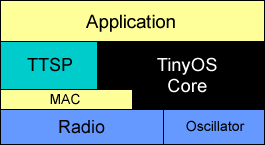
\includegraphics[scale=0.7]{./images/02-ttsp-hwsf_arch.png}
\end{center}
\caption{TTSP design goals.}
\label{designgoals}
\end{figure}

\subsection{Requirements}
%-----------------------------------------------------------
% keywords: requirements
%-----------------------------------------------------------
Here, follows a broad set of requirements that tries to address the time synchronization problem in WSNs. These requirements shall be fulfilled by a time synchronization protocol for WSNs. The requirements of a WSN protocol greatly differ from those found on a classic wired network, mainly due to its resources constraints. A WSN is often found with scarce resources at its disposal and it may be deployed on a hostile environment, where robustness to sensor node and communication link failures is also a key factor.

\subsubsection{Energy efficiency}
As with every other type of WSN protocol, a time synchronization protocol should take into account the limited energy resources that are available to the sensor nodes.

\subsubsection{Scalability}
A time synchronization protocol should not be limited to the  number of sensor nodes in the network. It should scale well with increasing number of sensor nodes.

\subsubsection{Precision}
A time synchronization protocol should fulfil the precision requirements of the applications. The need for precision or accuracy, may vary significantly depending on the specific application and the purpose of synchronization.

\subsubsection{Robustness}
Taking into account the energy constraints, the hostile environment that the WSN may be deployed and the volatile link quality of the communications in WSNs, it is expected that sensor nodes die, be removed from the network, or simply be unable to communicate between themselves for periods of time. The time synchronization protocol should remain valid and functional in the network, in case of failure of one or few of its sensor nodes. 

\subsubsection{Lifetime}
The time synchronization protocol in a WSN may provide time synchronization to its sensor nodes in a instantaneous fashion and act as long as the lifetime of the network.

\subsubsection{Scope}
A time synchronization may provide time synchronization to a local subset of the sensor nodes in the WSN, or a global time synchronization to all of the sensor nodes in the network.

\subsubsection{Cost and size}
The time synchronization protocol for WSNs should be developed with limited cost and size in mind. Adding dedicated hardware to every sensor node in the WSN for time synchronization may not be an option, as it can increase the cost for every sensor node and its overall size.

\section{Cross-layer interfaces}
%-----------------------------------------------------------
% keywords: cross-layer interfaces
%-----------------------------------------------------------
In order to fulfil its purpose, TTSP offers the application developer a specialized interface that, while still maintaining some similarities with conventional time synchronization protocol interfaces, has some special nuances that must be carefully taken into consideration. Mainly, the fact that, the cross-layer client of TTSP shall declare its tolerable threshold for time precision error, and/or its maximum synchronization period. The most relevant commands and events are illustrated in Figure \ref{crosslayer}.

\begin{figure}[!htb]
\begin{center}
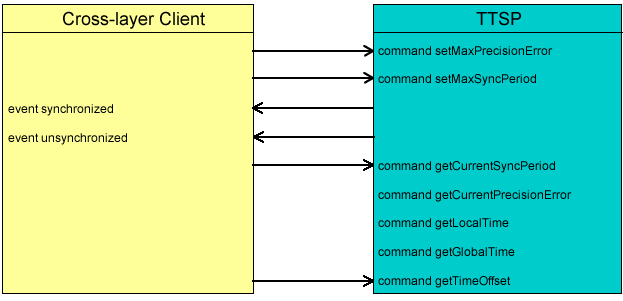
\includegraphics[scale=0.5]{./images/06-ttsp-crosslayer.png}
\end{center}
\caption{Cross-layer interfaces.}
\label{crosslayer}
\end{figure}

\section{System architecture}

%-----------------------------------------------------------
% keywords: system architecture
%-----------------------------------------------------------
As previously explained, TTSP allows its cross-layers applications to declare their time precision requirements, by stating their tolerable time precision error. These requirements are to be managed by an adaptive synchronization layer, which encapsulates all the adaptive logic, that is, contains the adaptive algorithm, maintains the state of the current precision error, synchronization period, reference clock node and requirements declared by its clients. This adaptive synchronization layer operates over two other classic synchronization layers: pair-wise synchronization and network-wide synchronization. Each one of these two layers encapsulates their own synchronization logic, that is, implement the algorithms for pair-wise and network-wide synchronization, and both are controlled by the adaptive synchronization layer. These two layers export a set of commands and events that allow the upper layer to take full control of the time synchronization techniques. This modular architecture for TTSP, allows one to easily substitute the pair-wise or network-wide synchronization algorithms and keep using the adaptive synchronization as long as they implement the set of commands and events that are used by the adaptive synchronization layer. Following a bottom-up approach, each one of these layers will be individually detailed below in Figure \ref{ttsparch}.

\begin{figure}[!htb]
\begin{center}
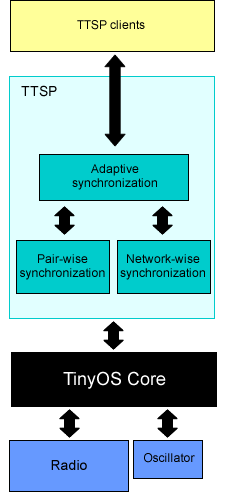
\includegraphics[scale=0.5]{./images/05-ttsp-design_goals.png}
\end{center}
\caption{TTSP architecture.}
\label{ttsparch}
\end{figure}

\subsection{Pair-wise synchronization}
%-----------------------------------------------------------
% keywords: pair-wise synchronization
%-----------------------------------------------------------
For pair-wise synchronization, TTSP uses a Sender-to-receiver message exchange scheme, mainly due to its low complexity and less complex requirements. This pair-wise synchronization will be refreshed periodically. By using a MAC-layer time-stamping with an approach like Sender-to-receiver, the high delay uncertainty found in this type of approach clearly decreases when compared with a Receiver-to-receiver. Making it a good choice instead of a Receiver-to-receiver with its inherent complexity.  By combining multiple estimates of the local time of a remote sensor node and using interpolation techniques it will be possible to compensate local clock skews.

\subsubsection{Synchronization through message exchange}
%-----------------------------------------------------------
% keywords: message exchange
%-----------------------------------------------------------
Assuming a Sender-to-receiver scheme, we're talking about synchronization between two or more nodes that are in the radio range of the sender and are able to exchange messages between themselves. Time synchronization between these nodes means that the nodes establish some relationship between their local clocks. The solution is for the sender to send a message containing a local time stamp to one of its neighbouring nodes, thus allowing the receiving node to synchronize with the senders clock. Although we've talked about only one receiving node, we can extend this message exchange to every receiving node that is in the radio broadcast area of the senders node.\\
Once a receiving node receives a synchronization message from the sender, he is now in possession of the senders local clock together with a local time stamp taken from of its own local clock of when the message was received. The receiving node is now able to calculate the offset between both clocks, and successfully adjust its logical clock to match with the senders local clock. This pair of  clock time stamps are commonly known as a synchronization point. Synchronization points are collected by the receiving nodes when a sender broadcasts its local clock.\\
In Figure \ref{syncmsg} it is possible to understand the synchronization process between two nodes through message exchange. Node i sends a message with a time-stamp of its local clock to node j. This process easily allows the receiving nodes to become aware of node i local clock.

\begin{figure}[!htb]
\begin{center}
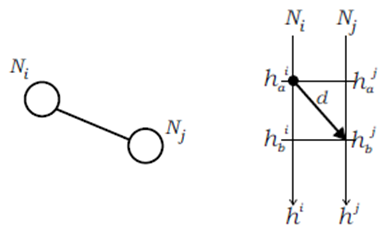
\includegraphics[scale=0.8]{./images/24-ttsp-sync_msg.png}
\end{center}
\caption{Two nodes synchronizing through message exchange.}
\label{syncmsg}
\end{figure}

But one problem persists with this technique, the receiving node cannot determine the exact delay of the message. It only knows for certain that the time-stamp of the local clock of the sender node was taken before he had received the message. Typically the uncertainty of the delay present in this message exchange can be decomposed in the following delays:

\begin{itemize}
\item the send time, lasting from when the application issues the send command to when the node actually starts trying to send; it is caused by kernel processing, context switches, and system calls, and hence varies with the current system load.
\item the (medium) access time, lasting from when the node is ready to send to when it actually starts the transmission; this is the time that is spent waiting for access to the wireless channel, and hence depends on the current network load.
\item the transmission time, which is the time taken to actually transmit the message, which depends only on the length of the message being transmited.
\item the propagation time, which is the time it takes for the radio signal to travel from the sender to the receiver; it is constant for any pair of nodes with constant distance, and is negligible compared to the other delay components in wireless sensor networks (since distances are small and radio signals travel very fast).
\item the receive time, lasting from the reception of the signal to the arrival of the data at the application.
\end{itemize}

Of all of these, only the transmission and the propagation time are deterministic. The send and receive time (and especially the uncertainty about them) and eventually the access time uncertainty can be reduced by implementing the time-stamping of outgoing and incoming messages at a very low level, for instance in the MAC layer.

\subsubsection{MAC-layer time-stamping}
%-----------------------------------------------------------
% keywords: MAC-layer time-stamping
%-----------------------------------------------------------
To minimize the delay uncertainty of the synchronization through message exchange, the use of time-stamping at the MAC-layer is essential, since it immediately limits three sources of delay uncertainties: access, transmit and receive times. In this case, the main message exchange delay comes from transmission and reception times at the radio chips. These delays can be further decomposed into 1) interrupt handling time, which is the delay between the radio chip raising and the micro-controller responding to an interrupt; 2) encoding time, which is the time it takes for the radio chip to encode and transform the message into a radio wave; 3) decoding time, which is the time for the radio chip at the receiver to transform the radio wave back into binary data; and 4) byte alignment time, which is the delay at the receiver to synchronize with the byte boundary at the physical layer. Thus, by using multiple time-stamps at the MAC-layer, when sending and receiving messages, it is possible to eliminate the jitter of interrupt handling and encoding/decoding times. 

\subsubsection{Synchronization rounds}
%-----------------------------------------------------------
% keywords: synchronization rounds
%-----------------------------------------------------------
Typically, two local clocks do not run at exactly the same speed. Therefore time synchronization has to be refreshed periodically, that is once these two clocks synchronize, they'll eventually start to drift apart from each other, mainly due to the sole characteristics of the hardware clock, the crystals oscillator might not have the same oscillating frequency, but also due to environmental conditions such as pressure and temperature which might affect the oscillating frequency of the crystal clocks. Thus, time synchronization in rounds becomes a continuous process, rounds follow each other seamlessly. So for every synchronization round a receiving node is able to collect one synchronization point. The duration of the round, or more commonly known as the synchronization period, depends on the available error budget and the amount of relative clock skew between the two clocks. As we will see below, one of the key factors in the adaptive synchronization will be adapting this synchronization period to satisfy the time precision error needed by the cross-layer applications.

\subsubsection{Skew compensation by combining multiple estimates}
%-----------------------------------------------------------
% keywords: skew compensation
%-----------------------------------------------------------
Although the synchronization may be done in rounds, through periodical broadcasted messages, one might take into consideration clock skew compensation techniques, which would minimize the offset from the two clocks in between synchronization points. As previously said, it's typical to find that different nodes have different clock skews, which is true, since the crystal used by the hardware clock might oscillate with a slight different frequency on each node, and thus, drift apart from each other at different rates.\\
In order to evaluate the clock skew between the nodes clocks, some tests were carried out on an already deployed test-bed, Tagus-SensorNet. The test involved six nodes and lasted for twenty-four hours. One node, the sink, was used as the clock reference for the remaining five nodes, these were initially synchronized at the beginning of the test and their clock skew was analysed during the following hours, that is, every node was allowed to collect only the initial synchronization point. The obtained results can be seen in Figure \ref{tsnclockskewchart}.\\

\begin{figure}[!htb]
\begin{center}
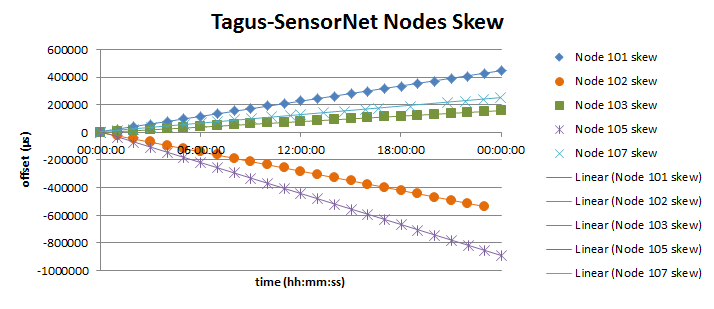
\includegraphics[scale=0.5]{./images/07-ttsp-tsn_skew.png}
\end{center}
\caption{Tagus-SensorNet nodes clock skew over 24 hours.}
\label{tsnclockskewchart}
\end{figure}

It's clear that once synchronized, each node starts to drift apart from the reference clock at a different rate. In order to get an approximated value of this rate, linear regression was used to find the best line that fits the collected dataset. The clock skews from each node were then obtained, and are shown in Table \ref{tsnclockskewtable}. 

\begin{table}[!htb]
\begin{center}
\begin{tabular}{|c|c|}
\hline
Node & Skew (ppm)\\ \hline
101 & 5,074 \\ \hline
102 &  -6,5 \\ \hline
103 &  1,797 \\ \hline
105 &  -10,376 \\ \hline
107 &  2,875 \\ \hline
\end{tabular}
\caption{Tagus-SensorNet nodes clock skew express in parts per milllion.}
\label{tsnclockskewtable}
\end{center}
\end{table}

Linear regression is the most widely used technique to predict the clock skew of a nodes clock, thus, allowing one to compensate for its clock skew with regard to its reference clock. As can be seen in Figure \ref{tsnclockskewerror}, the error obtained while predicting the above clock skews using linear regression assumes a bell-shaped distribution with its centre at 0 microseconds and a maximum error value of 57 microseconds.\\

\begin{figure}[!htb]
\begin{center}
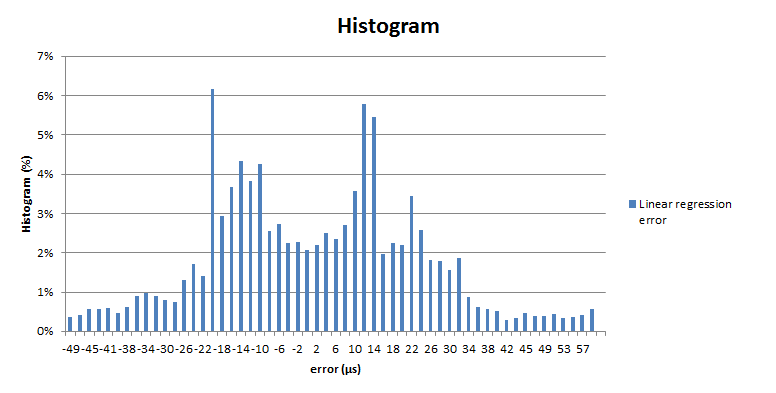
\includegraphics[scale=0.5]{./images/08-ttsp-tsn_histogram.png}
\end{center}
\caption{Error distribution while using linear regression to compute clock skews on Tagus-SensorNet.}
\label{tsnclockskewerror}
\end{figure}

This technique has a single parameter, that is the number of synchronization points that are accounted for when computing the clock skew. A large number of synchronization points can improve the regression quality, but requires a large amount of memory and might demand a considerable amount of processor occupation when done periodically. Linear regression implicitly allows one to compensate for the clock skew, but the clock skew is often variable during time, thus the postulated linear relationship between both clocks does not describe reality very well. In such situation, the number of samples accounted for should be small enough in order to minimize possible errors. Linear regression can be computed on-line, computed whenever a new sample is available. As we later experienced, with the adaptive mechanism being used, and synchronization periods being incremented and decremented between synchronization rounds, the best number of synchronization points found to adapt to the different rate at which samples would be collected, is between 4 and 8 samples.\\

\subsection{Network-wide synchronization}
%-----------------------------------------------------------
% keywords: network-wide synchronization
%-----------------------------------------------------------
For network-wide synchronization, the approach used for synchronization throughout the network is a master-slave scheme mainly also due to its low complexity and easy prediction of its behaviour while comparing to a peer-to-peer approach. The master will broadcast its local time to its neighbours, once these neighbours get synchronized with this master, they will then also start broadcasting to their neighbours.  In order to provide some redundancy to the master and easily adapt to network topology changes, a simple master election algorithm will ensure that a new root is elected once the previous one has cease to broadcast its local clock.

\subsubsection{Controlled flooding of broadcasted messages}
%-----------------------------------------------------------
% keywords: flooding
%-----------------------------------------------------------
The elected reference clock node, more commonly known as the root node, to which the whole network is being synchronized, keeps broadcasting its local clock within a certain period. Every other node that is within the broadcast radius of the root node can receive time-stamped messages from him, and collect synchronization points. When a node has collected enough synchronization points, he will be able to successfully compensate its clock skew with regard to the root node. By then, his in possession of the offset and the skew between both clocks. That node is considered synchronized with the root node and is now also able to start broadcasting its logical clock to its neighbouring nodes. The continuation of this process will eventually reassemble to a flooding of synchronization messages throughout the network. This flooding process takes advantage of the promiscuous communication medium that these wireless nodes use, allowing for a network-wide synchronization without a logic level hierarchy that many of the available time synchronization protocols for WSNs use.

\subsubsection{Master election mechanism}
%-----------------------------------------------------------
% keywords: master election mechanism
%-----------------------------------------------------------
One of the most critical problems found when using a master-slave approach for network-wide synchronization is that, the whole time synchronization process in the network, has one single-point of failure, that is the root node. It is important to introduce some redundancy in the network-wide synchronization process in case the root node for any technical reason fails or its broadcasted messages are subject to a permanent or temporary radio interference. The solution is to use a master election mechanism whenever the current root nodes is absent of the network. The root node is considered absent if for any reason the receiving nodes fail to collect a specific number of  synchronization points, which translates itself to a specific number of missed synchronization rounds. In order to prevent early master elections, the receiving nodes are configured to tolerate only a number of missing synchronization point, these optimal numbers as we later experienced, are from 3 to 4. These values are justified from a series of tests conducted in Tagus-SensorNet, in which lower values would trigger an early master election, which was caused by messages not being received by some of the receiving nodes, and a higher value would induce a slow detection of the master failure, thus a slower response and nodes would eventually be subject to variable time precision errors during that time.\\

Once the root node is declared absent from the network, the remaining nodes need to agree on a replacement for the root node. One here, could think of the hardware capabilities that could differentiate a node to be elected as replacement of the absent master, but since most WSNs test-beds, like Tagus-SensorNet lack some heterogeneity in hardware capabilities and platforms, that wouldn't make any differentiation. One solution would be to give priority to nodes that have plenty energy resources at their disposal, but that would almost always end with giving priority to nodes that are at the edges of the network and eventually create deep multi-hop chains between synchronizing nodes. The chosen solution for this priority, is the less complex and most predictable one. Nodes are elected as replacements for the root node by their logical identification. Every node gives high priority to a root node with a lower identification while synchronizing. That is, once the previous root node is declared absent from the network, each node declares itself as a possible candidate for being a replacement for the root node by starting broadcasting their local clock. Nodes will start a pair-wise synchronization with the self-elected root node that has the lower identification. Once they get synchronized with the new root node, they will also start broadcasting their logical clock. This broadcast contains the identification of the root node, so that in multi-hop scenarios, every node gets updated and synchronized with the new master.


\subsection{Adaptive synchronization}
%-----------------------------------------------------------
% keywords: adaptive synchronization
%-----------------------------------------------------------
By now, we've seen, that in order to maintain a long-term time synchronization among nodes, a periodic re-synchronization is needed, otherwise the timing of different nodes would drift apart as time passes. Thus, one needs to take into account that a less frequent re-synchronization requires a lower number of exchanged messages, thus, eventually lesser energy consumption by the sending and receiving nodes, but ultimately leads to a larger synchronization error, that is, time precision error. While a more frequent re-synchronization leads to a smaller time precision error but requires more energy. There is clearly a trade-off between energy expenditure and the achieved time precision error. The proposed adaptive synchronization layer shall find the minimum re-synchronization frequency (or equivalently maximum re-synchronization period) that can meet the desired  synchronization precision.\\
Therefore the adaptive synchronization layer is necessary to dynamically determine the re-synchronization period to be used in each round of synchronization based on the needed time precision error.

\subsubsection{Time precision error}
%-----------------------------------------------------------
% keywords: time precision error
%-----------------------------------------------------------
The adaptive synchronization must have knowledge of the required time precision error. As previously said, this precision error is declared by the cross-layer clients. Once the adaptive layer knows this value, it now needs to know how to systematically measure the current achieved time precision error. This measure is done at both the sender and the receiver. Each one should monitor this parameter in order to actuate over it.\\
The sender, more specifically the root node which is being used as the reference clock, has the responsibility of adjusting the synchronization period based on the precision error calculated from the broadcasts of the receiving nodes, once they get synchronized. One of the advantages of having a promiscuous physical medium and the fact that exchanged messages are broadcasted on it, is that the root node can listen to its synchronizing nodes broadcasts and measure the precision error of the synchronization messages they broadcast. In a multi-hop scenario these precision errors are obtained through relayed messages by the intermediary nodes. These intermediary nodes, which by then are already synchronized with the root node and aware of the time precision requirements are able to filter messages in case the calculated precision error is acceptable. Thus, in a multi-hop scenario the intermediary nodes have the responsibility of letting the root node know about unacceptable precision errors in the edges of the network.\\
On the other side, the receiver has a lesser significant responsibility but still important of managing the synchronization points already collected and employ filtering techniques on them, in order to assure an acceptable time precision error. This management is needed since, while adjusting to a new synchronization period, the already collected number of samples might induce some small precision error when calculating the logical clock time.

\subsubsection{Synchronization period}
%-----------------------------------------------------------
% keywords: synchronization period
%-----------------------------------------------------------
As previously said, only the root node has the responsibility of adjusting the synchronization period. The initial synchronization period is statically pre-configured on all nodes, and should reflect a period that is known to be safe to start with. The following synchronization periods to be used by the root node are adjusted by the adaptive algorithm, which reflect the current time precision error. This adaptive adjustment is made on the sole basis of the current time precision error. The adjustment is made using a \ac{MIMD} strategy. The concept is straightforward, if the current time precision error is larger than  the requested time precision, it means that the synchronization period is too high, therefore the synchronization period should decrease by a certain factor. On the other hand, if the time precision error is smaller than the requested time precision error, that translates into a lower synchronization period, and thus, it could be increased by a certain factor. This procedure is seen as a transition state, in which there is no knowledge about the best synchronization period to be used, which are mainly influenced by the network topology (multi-hop distances), node crystals and the environment itself. After the adaptive algorithm stabilizes, that is, after it found at which period it achieves an acceptable time precision error on all nodes, it then stops adjusting the synchronization period. This adaptive algorithm can be best described by a finite-state machine, depicted in Figure \ref{statemac}  which is composed by three distinct states. 

\begin{figure}[!htb]
\begin{center}
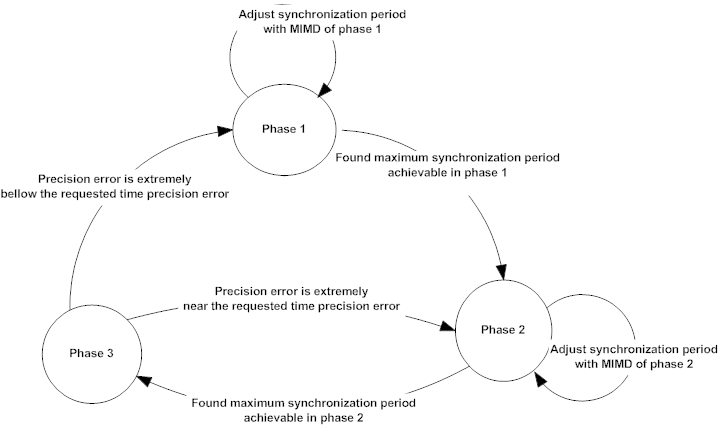
\includegraphics[scale=0.5]{./images/25-ttsp-machine_state.png}
\end{center}
\caption{Finit-state machine for the synchronization period adjustment algorithm.}
\label{statemac}
\end{figure}

The finite-state machine used in the adaptive algorithm has three distinct phases. In each phase of this finite-state machine the synchronization period is adjusted. Although, each phase is characterized by having its particular \ac{MIMD} granularity level, starting with a lower \ac{MIMD} granularity level in phase 1 while finishing with a higher \ac{MIMD} granularity level at phase 3. The transition conditions on the first two phases are the same, with the sole objective to quickly assess the maximum synchronization period that is possible to achieve under the given conditions, that is, to find the maximum synchronization period that is possible to be achieved with that \ac{MIMD} granularity level while maintaining an acceptable precision error. For the first and second phase, once this maximum synchronization period is obtained, there is a transition to a phase with a higher \ac{MIMD} granularity level. On the third and last phase, the \ac{MIMD} granularity level is sufficient high that only minimal changes to the synchronization period are taken place, this can be seen as entering a stabilization process in the adjustment of the synchronization period. The transition conditions in this phase differ from the previous two, since the objective here is to guarantee that significant precision error changes with the achievable time synchronization period are mitigated by finding a new best suitable time synchronization period.

In order to support the better explanation of this finite-state machine and the underlying decisions taken by the synchronization period adjustment algorithm, a flowchart of every decision and action taken by this algorithm can be seen Figure \ref{flow} followed by a detailed explanation of each phase.

\begin{figure}[!htb]
\begin{center}
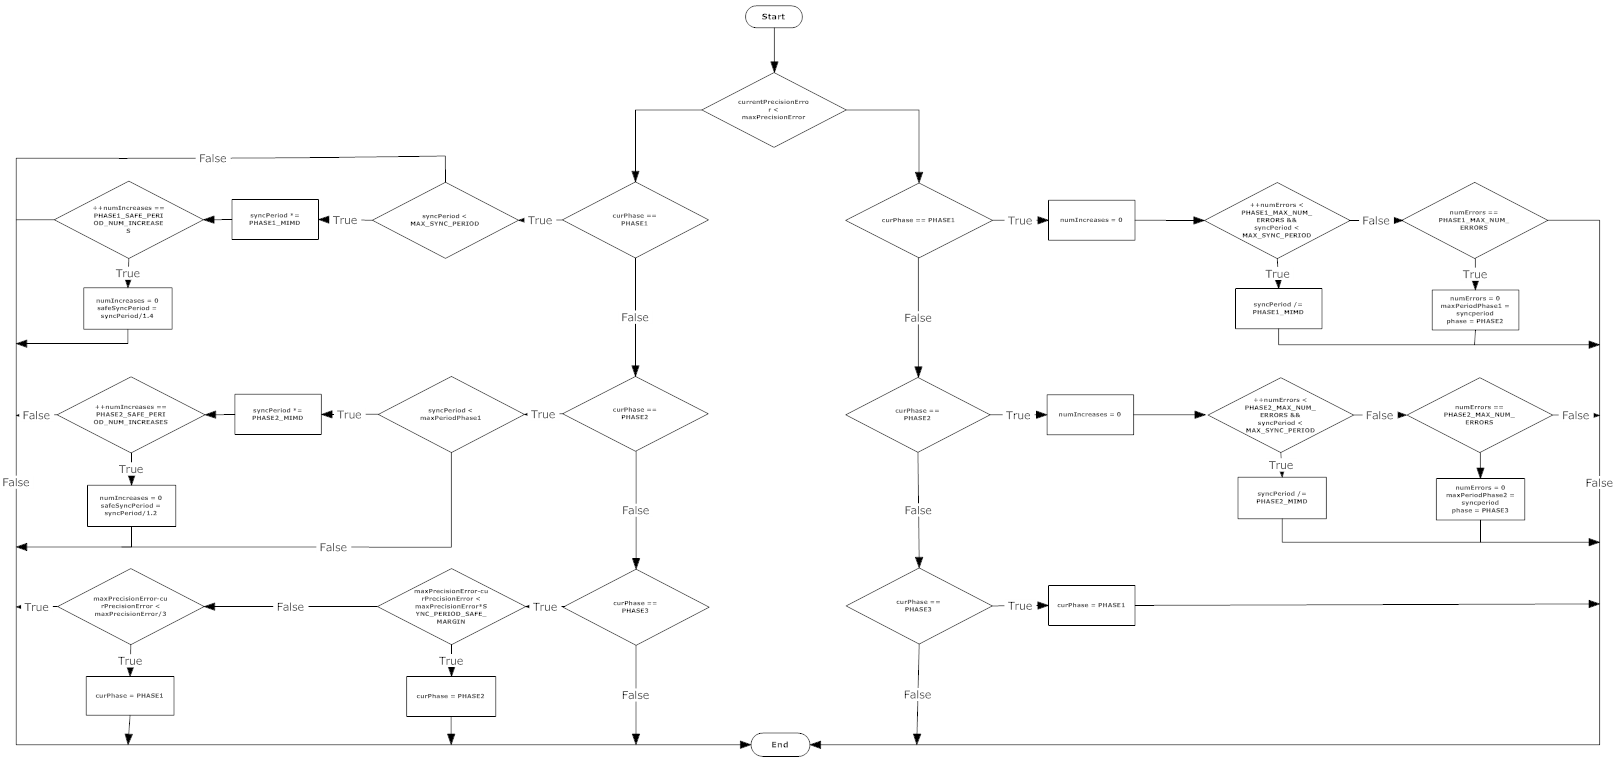
\includegraphics[scale=0.4,angle=90]{./images/26-ttsp-flowchart.png}
\end{center}
\caption{Detailed flowchart of the synchronization period adjustment algorithm.}
\label{flow}
\end{figure}

\clearpage

The first and initial phase, known to be as phase 1, is triggered on the root node after the first synchronization message from one of its receiving nodes is received, that is, once one neighbouring node gets synchronized and starts to broadcast its logical clock time. From that on, and on every synchronization message received in a synchronization round from its synchronized neighbours, the root adjusts the synchronization period to meet the required time precision error. The root node filters synchronization messages by its synchronization round identification, so that it only adjusts the synchronization period once in a synchronization round. Although, there are cases in which one node has an acceptable error, but another don't, in this case, the root needs to filter messages by synchronization rounds but also take into consideration the time precision error of the node, eventually giving priority to adjustments that keep the overall time precision error lower. For every two consecutive period increases, the algorithm records a safe period, which it will use as a fall-back when it receives a non-consecutive number of synchronization messages with an unacceptable precision error and needs to drastically decrease the synchronization period. The MIMD granularity used in this phase is typically higher than the other remaining phases, since there is no knowledge at that moment from the conditions of the network. The transition from this phase is done after a certain number of non-consecutive synchronization messages with a time precision higher than the accepted. When transitioning from this phase, the adaptive algorithm has the knowledge of the maximum synchronization period that it can sustain for the given network conditions. As said, this transition will be made after the maximum synchronization period is known, this will typically involve achieving a higher time precision error, which will result in a decrease in the time synchronization period to a known safe period, as previously explained. The next phase, will take this knowledge into consideration.

The second phase of the adaptive algorithm, known as phase 2, is somehow similar with the first phase, it also can be described as a discovery phase, but now with the difference that we know the maximum synchronization period that can be achievable under an acceptable precision error, thus the MIMD granularity used in this phase is smaller than the used on the previous phase, since we're are interested in maximizing the synchronization period closer to the previous known maximum synchronization period but without the precision errors. Like in the previous phase, the algorithm quickly reacts to small variations of the achieved time precision error in order to keep it under the required precision. This phase is also considered a transition state, that is, the synchronization period can still fluctuate significantly between the two distinct thresholds that it knows, the safe synchronization period and the maximum synchronization period obtained from the previous phase. The transition from this phase is done after a certain number of consecutive increases and a decrease or a certain number of decreases and an increase.

The third and last phase of the adaptive algorithm, phase 3, can be considered as a stabilization phase, since once in this phase the current synchronization period is considered safe and lower the maximum synchronization period where the unacceptable time precision errors were detected. In this phase, the MIMD granularity is very small since for most cases the precision error should be within the required thresholds and not be subject to high variations. This phase can be grossly characterized by a steady synchronization period. Nonetheless, if by any means, the time precision error keeps getting close to the threshold of the requested time precision error for a long period of time, that is, a certain number of synchronization round, a transition to phase two will be made, since it is considered that the current synchronization period is not suitable any more. The same procedure is made for when the time precision error is well below the requested time precision error and close to zero, but instead, a transition will be made to phase one, because of its higher MIMD granularity.

\subsubsection{Fast synchronization}
%-----------------------------------------------------------
% keywords: fast synchronization
%-----------------------------------------------------------
One needs to take into consideration that when adaptively adjusting the synchronization period in a network of sensor nodes, new nodes might be added to the network and it might be requested that they should get as quickly as they can synchronized with the rest of the network nodes. This is somehow inefficient while on a large synchronization period, since typically a node needs to collect a certain number of synchronization points before it gets synchronized with remain nodes. Thus, on those cases the new node would have to wait for N times the large synchronization period, where N is the number of necessary synchronization points, which would consume a considerable amount of time and  has proven not to be acceptable in networks which might have nodes being turned off for maintenance and added back again with some high frequency. For those cases a fast synchronization mechanism was introduced to quickly detect and synchronize new nodes in the network. The concept is that a node will discard synchronization messages that contain a large synchronization period, thus eventually declaring itself the root node since all synchronization messages from possible root nodes have been discarded. Once it declared itself the root node, it will start to broadcast with its identification which will be received by neighbouring nodes which are already synchronized with the correct root node. Upon receiving a synchronization message from a root that is not his root and not in conditions to be a root, the receiving node will trigger a fast synchronization mechanism which will broadcast a consecutive number of synchronization messages within a short period of duration. The new node will then be aware of the real root node and also be able collect the necessary synchronization points in order to synchronize with him. The consecutive number of messages are sent using the initial synchronization period, which is quite small compared to the possible synchronization period that might be in use, thus, this procedure only takes up to N times the initial synchronization period, which by convention is much smaller than the larger synchronization period.\\

To briefly summarize TTSP architecture, it can be best seen as a set of common techniques that are used by many of the existent time synchronization protocols, but with the exception, that here, they are embedded in an adaptive mechanism in order to meet specific requirements that are demand by TTSP clients. Thus, these tools are to be used with regard to the desired time precision. They are used by the adaptive mechanism in order to cope with the effort necessary to achieve the desired time precision. Although many of these techniques are broadly used by other time synchronization protocols, most of them required a significant number of modifications or complements in order to be usable in a adaptive fashion, for example, the compensation skew technique, which requires a specific number of samples and a better management and filtering of these samples while adjusting the synchronization period.\\

\cleardoublepage

\chapter{TTSP Implementation}

%-----------------------------------------------------------
% keywords: Reference implementation
%-----------------------------------------------------------
As previously said, a reference implementation was also developed. This intention had the purpose of demonstrating that such architecture could be implemented but also to validate and evaluate its effectiveness and efficiency that can be achieved with it. This reference implementation was developed on the Crossbow MICAz hardware platform which executed the TinyOS platform, which is mainly described for being very low resource demanding and having an event-centric and a modular component architecture. TTSP was implemented as a TinyOS library, thus, it is made available to every other component of the operating system (including the already available MAC protocols) and the upper lying TinyOS application developed by the user. 

\setcounter{secnumdepth}{2}
\section{Development hardware and software platform}
%-----------------------------------------------------------
% keywords: Development hardware and software platform
%-----------------------------------------------------------

\subsection{Hardware platform}
%-----------------------------------------------------------
% keywords: Crossbow MICAz 
%-----------------------------------------------------------
TTSP reference implementation has been developed on the TinyOS 2.x software platform, and has been primarily tested on Crossbow MICAz sensor nodes \cite{crossbow04}. The Crossbow MICAz is a commercially available sensor platform that couples an 8-bit AVR RISC microcontroller, the Atmel ATmega128L \cite{atmel08}, with an IEEE 802.15.14 Zigbee-ready transceiver, the Chipconn CC2420 \cite{cc04}. The use of this platforms, in itself, is a challenge to overcome, especially due to the reduced amount of available memory on the MICAz sensor node (4 kB of SRAM).\\
The relatively limited amount of memory on this type of hardware platform posed some implementation challenges to the developer. One most take into account that the developed TTSP library will eventually be used in conjunction with an application, so in order not to limit even more the development of applications regarding memory size, developed libraries must try to squeeze its size to the maximum.\\
As we will see next, most of the software code developed over this platform has been re-factorized in order to guarantee its minimum implementation footprint.

\subsection{Software platform}
%-----------------------------------------------------------
% keywords: Monolothic architecture
%-----------------------------------------------------------
TinyOS, is an open-source operating system initially developed at the University of California, Berkeley. This operating system was specifically designed to work on embedded systems with very severe computational constraints, such as those found in WSNs, and has, since then, become the de facto standard operating system for several WSN platforms.\\
TinyOS combines flexible, fine-grain components with an execution model that supports complex yet safe concurrent
operations. Its built from a set of reusable components that are assembled into an application-specific system. Like the
applications, the solution is event-centric. The normal operation is the reactive execution of concurrent events. This event-driven concurrency model is based on split-phase interfaces, asynchronous events, and deferred computation called tasks.
These component and execution models avoid the use of complex structures for scheduling and locking mechanisms between
tasks lowering the need for memory resources.\\
This specialized architecture is further supported by a specialized C-like programming language, with which all TinyOS components must be programmed, called nesC \cite{gay03}. The application is statically linked with the kernel to create a
complete image of the system at compile-time. After linking, modifying the system is not possible.

\begin{itemize}
\item Limited resources
\item Flexibility
\item Concurrency
\item Power management
\end{itemize}

The module of construction of TinyOS is built around these four main goals and it encompasses all the general features that
are expected of a sensor node operating system to perform effectively and also maximize performance.
Additionally, TinyOS provides a powerful simulation environment, TOSSIM \cite{levis03} \cite{lee03}, which enables the simulation of entire WSNs using the same source-code that is used on real sensors.

\section{Implementation considerations and complexity}
%-----------------------------------------------------------
% keywords: Implementation details and complexity
%-----------------------------------------------------------
As previously said, TTSP was implemented as a library that can be included and used by any application. Its implementation follows a modular approach, in which, each of the three principles of synchronization logic used by TTSP are encapsulated in their own modules. This modular approach eases software development and its debugging. Additionally, as already stated here, it allows one to easily switch or modify the corresponding synchronization logic without breaking the remaining other logic blocks. The complexity aimed for TTSP's implementation development was to be minimal as possible. The chosen synchronization techniques are easily implemented and its simple behaviour (yet theoretical efficient) facilitates debugging.

\subsection{Implementation considerations}
%-----------------------------------------------------------
% keywords:
%-----------------------------------------------------------
Although the implementation of TTSP did not pose serious constraints to the proposed conceptual architecture, there are some important considerations to retain from this process, especially those that have a great impact on the overall performance of TTSP in real-life scenarios, whether it be the interfaces that the common developer will need to master in order to make their applications and MAC protocols aware of TTSP services or the synchronization period adjustment algorithm which is the core piece of TTSP and may be tunable/hackable in order to satisfy exquisite network topologies. Additionally, some implementation considerations are needed for non-trivial synchronization techniques.

\subsubsection{Interfaces}
%-----------------------------------------------------------
% keywords:
%-----------------------------------------------------------
Regarding the interfaces that are available to interact with TTSP, the most important one is AdaptiveTimeSync. This interface is exported to the application and MAC-layer protocol. The signature of the AdaptiveTimeSync interface is depicted in Figure \ref{adapttimeysnc}. This interface tells us that the clients of TTSP should implement both the synchronized and unsynchronized events while TTSP should implement all the remaining commands that are to be used.

\begin{figure}[!htb]
\begin{center}
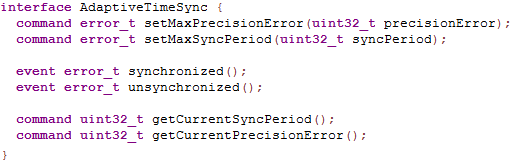
\includegraphics[scale=0.5]{./images/27-ttsp-code_interfaces.png}
\end{center}
\caption{AdaptiveTimeSync interface.}
\label{adapttimeysnc}
\end{figure}

As explained in the previous chapter, these interfaces are exported by the adaptive synchronization logic implementation. With regard to memory constraints (in this case heap memory size) and number of CPU instructions, the remaining interfaces are exported from the pair-wise and network-wide synchronization logic modules. This avoids unnecessary memory usage and increases the execution speed overall of the following commands.\\
The following interface that is exported to the application layer and MAC-layer is a more simpler to use but still deeply important, as it allows the application or the MAC-layer protocol to be aware of the logical clock. This interface can be found in Figure \ref{globaltime}.

\begin{figure}[!htb]
\begin{center}
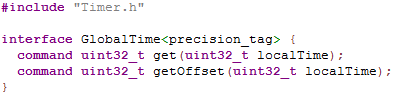
\includegraphics[scale=0.5]{./images/28-ttsp-code_interfaces2.png}
\end{center}
\caption{GlobalTime interface.}
\label{globaltime}
\end{figure}

The last remaining interface that can be seen in Figure \ref{timesyncinfo} allows the application to get some knowledge whether it is the root or if not, the root node to which the node is synchronized.

\begin{figure}[!htb]
\begin{center}
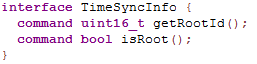
\includegraphics[scale=0.5]{./images/29-ttsp-code_interfaces3.png}
\end{center}
\caption{TimeSyncInfo interface.}
\label{timesyncinfo}
\end{figure}

An overall view of the wiring of the AdaptiveTimeSyncP and its components and interfaces can be viewed in Figure \ref{compwiring}.

\begin{figure}[!htb]
\begin{center}
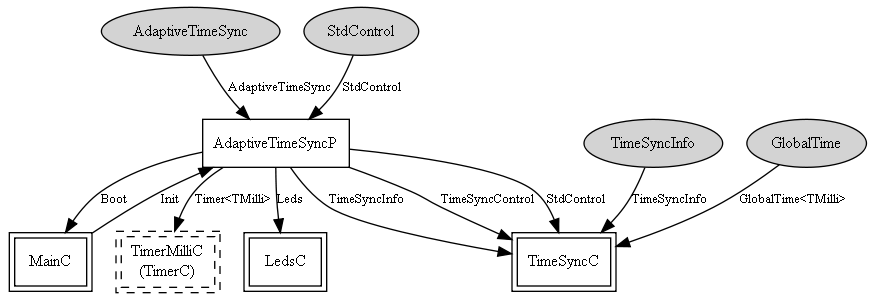
\includegraphics[scale=0.4]{./images/30-ttsp-interface_wiring.png}
\end{center}
\caption{Wiring of AdaptiveTimeSyncP component and its application and MAC-layer interfaces.}
\label{compwiring}
\end{figure}

On the other side, we have another special interface which interacts between the AdaptiveTimeSyncP component and the pair-wise and network-wide synchronization logic (which is encapsulated in TimeSyncP component), the TimeSyncControl interface. This special and more complex interface is the glue between the adaptive time synchronization and the pair-wise and network-wide synchronization. This interface exports control of the underlying mechanisms for pair-wise and network-wide synchronization to the adaptive time synchronization logic component. The Figure \ref{timesynccontrol} shows an excerpt of the commands and events that this interface exports.

\begin{figure}[!htb]
\begin{center}
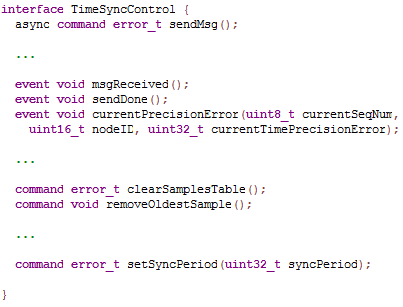
\includegraphics[scale=0.5]{./images/36-ttsp-code_interfaces4.png}
\end{center}
\caption{TimeSyncControl interface.}
\label{timesynccontrol}
\end{figure}

Finally, an overview of the wiring of the TimeSyncP and its components and interfaces can be viewed in Figure \ref{timecomp}.

\begin{figure}[!htb]
\begin{center}
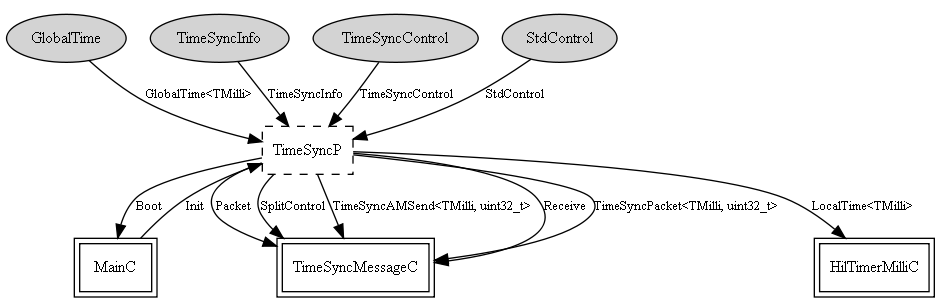
\includegraphics[scale=0.4]{./images/35-ttsp-interface_wiring2.png}
\end{center}
\caption{Wiring of TimeSyncP component and its interfaces.}
\label{timewiring}
\end{figure}

\subsubsection{MAC-layer time-stamping}
%-----------------------------------------------------------
% keywords:
%-----------------------------------------------------------
Typically, in TinyOS neither the time of invocation of the send command, nor the time of signalling of the sendDone event can be used to estimate, without significant jitter, the time when the packet was transmitted. Similarly, the time of occurrence of the receive event cannot be used to reliably estimate the time of reception. A straightforward way of message time-stamping while reducing the delay uncertainty, is to place these time-stamps when the message is being sent at the MAC-layer. TinyOS exposes a specialized interface which allows one to send messages while placing a time-stamp at the MAC-layer. Typically, this interface makes use of the \ac{SFD} interrupt handler on the CC2420 radio, which allows TinyOS to know when to place the time-stamp while sending the message through the radio.

The TimeSyncAMSend interface allows one for sending this time-stamp along with a message. This interface can be seen in Figure \ref{timesyncamsend}.

\begin{figure}[!htb]
\begin{center}
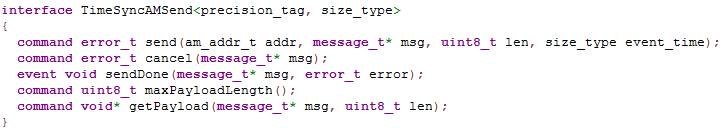
\includegraphics[scale=0.5]{./images/31-ttsp-mac_timestamp.png}
\end{center}
\caption{TimeSyncAMSend interface used for placing time-stamps on outgoing messages.}
\label{timesyncamsend}
\end{figure}

On the opposite side, that is on the receiving side, one can use the TimeSyncPacket interface to retrieve the time-stamp of the message. This interface is depicted in Figure \ref{timesyncpacket}.

\begin{figure}[!htb]
\begin{center}
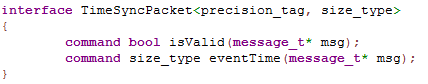
\includegraphics[scale=0.5]{./images/32-ttsp-mac_timestamp2.png}
\end{center}
\caption{TimeSyncPacket interface used for retrieving the time-stamp sent along with the received packet.}
\label{timesyncpacket}
\end{figure}
 
For example, when TTSP uses the TimeSyncAMSend.send command called with event time-stamp t1, it stores t1 and sends the packet to the MAC-layer. When the packet starts being transmitted over the communication medium, a corresponding hardware event is timestamped (an SFD interrupt). Let us denote this transmission time-stamp with t2. The difference of event time-stamp t1 and transmit time-stamp t2 is written into the designated time-stamp field in the payload of the packet (typically into the footer, since the first few bytes might have been transmitted by this time). That is, the information the packet contains at the instance when being sent over the communications medium is the age of the event (i.e. how much time ago the event had occurred).\\
In the receiver side, when the packet is received, it is timestamped with the receiver node's local clock at reception (e.g. with the time-stamp of the SFD interrupt). Let us denote the time of reception with t3. When the event time is queried via the TimeSyncPacket interface, the eventTime command returns the sum of the value stored in the designated time-stamp field in packet payload and the reception time-stamp, i.e. t1- t2+t3. This value corresponds to the time of the event in the receiver's local clock.

%\subsubsection{Skew compensation mechanism}%

\subsubsection{Synchronization period adjustment algorithm}
%-----------------------------------------------------------
% keywords:
%-----------------------------------------------------------
As previously said, the core piece of the adaptive approach of TTSP, is its synchronization period adjustment algorithm. This algorithm already has been explained in the previous chapter. The implementation of this algorithm was rather trivial, since it was modelled to be a finite-state machine. Implementing finite-state machine is accomplished by saving the current state and typically using a switch code block.\\
The Figure \ref{adaptivecode} depicts a code excerpt of the switch code block that implements the phase 1 of synchronization period adjustment finite-state machine.

\begin{figure}[!htb]
\begin{center}
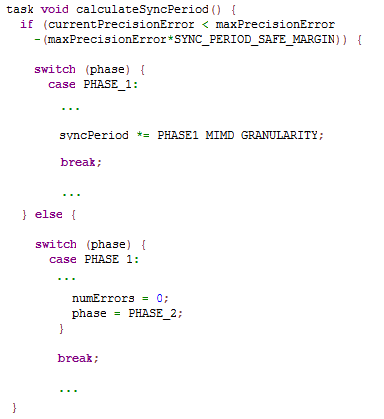
\includegraphics[scale=0.5]{./images/33-ttsp-adaptive_code.png}
\end{center}
\caption{Code excerpt of the switch code blocks used to implement phase 1 of the finite-state machine.}
\label{adaptivecode}
\end{figure}

The previous code block is executed whenever the root node has some feedback of the time precision of its neighbours. That is, when the pair-wise and network-wide synchronization components signal through an event the adaptive synchronization module. Thus, the code used for adjusting the synchronization period was placed on an individual task, due to the fact that its execution could starve other event signal flows in the operating system.

Once a new synchronization period is obtained, it is ready to be broadcasted by the root to the neighbouring nodes. In order to rapidly apply and start broadcasting the new synchronization period, the next synchronization round will be also recalculated in order to compensate those cases when the new synchronization period is less than the previous. The code developed for the described function is depicted in Figure \ref{adaptivecode2}.

\begin{figure}[!htb]
\begin{center}
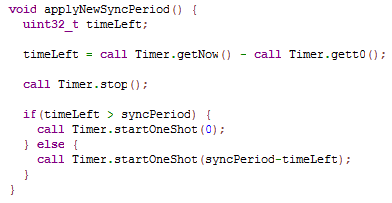
\includegraphics[scale=0.5]{./images/34-ttsp-adaptive_code2.png}
\end{center}
\caption{Code of the function to rapidly apply the new synchronization period.}
\label{adaptivecode2}
\end{figure}

\subsection{Implementation complexity}
%-----------------------------------------------------------
% keywords: Implementation complexity
%-----------------------------------------------------------
One of the goals set for TTSP was its ease of implementation, and verifying it was also one of the reasons leading to the development of this prototype. While ease of implementation is always a topic of subjective evaluation, some objective metrics can be presented.\\
The full implementation contains 10 components (configurations, modules and interfaces) and 1039 physical source lines of code (SLOC), excluding utilities and debugging functionality.
Regarding memory usage, an image ready to be flashed on a node compiled with a dummy application and TTSP, occupies 1903 bytes of RAM and 22487 bytes of ROM. So to speak, that leaves plenty of memory (both types) for the application developer.

\section{Redesign of Tagus-SensorNet}
%-----------------------------------------------------------
% keywords: Redesign of Tagus-SensorNet
%-----------------------------------------------------------
Regarding the test-bed itself and in parallel with TTSP development, there was an effort in redesigning Tagus-SensorNet to become more flexible in handling multiple and both software and hardware heterogeneous WSN's islands under one single software application development platform. The need came from the fact that multiple independent and many times strictly communication closed WSN's islands were starting to appear in Tagus-SensorNet (as a result of the increasing scientific interest that WSN is having at the moment). The previous architecture was unable to allow these new islands to communicate between themselves, the need to have multiple base-stations (sink nodes), each WSN island required its own base-station, but also do to the application development that much of the time was repeating already existent source code. This need led to propose a new architecture for Tagus-SensorNet which would also ease TTSP during its evaluation phase.

\subsection{Previous Tagus-SensorNet architecture}
%-----------------------------------------------------------
% keywords: Monolothic architecture
%-----------------------------------------------------------
Until recently, Tagus-SensorNet architecture had a monolithic structure which clearly was designed taking into account the limited set of hardware platforms commercially available at that time, the most popular operating system (TinyOS) and by that extent the limited number of available MAC-layer and network layer protocols. This architecture clearly satisfied its initial needs, that was to allow the application developer to interact with the nodes in a given application. Using this architecture the application developer tended to develop specifically TinyOS code on the nodes tightly coupled with the application itself. As we later became aware, much of the code was being repeated over time. And worst, many times this application code was being developed specifically for a given hardware platform.\\
Also, with the growth of the network, multiple WSN islands were being deployed to test and bench-mark a variety of protocols. The previous architecture clearly failed to allow these new islands to communicate between themselves if by any means they used a different MAC-layer protocol or a different radio frequency.

\subsection{Proposed and implemented changes}
%-----------------------------------------------------------
% keywords: 
%-----------------------------------------------------------
The proposed architecture decouples the embedded software running on the nodes hardware platform and the application itself. This way, it is possible to allow hardware and software heterogeneity in the network without implementing a MAC-layer or network layer protocol that is common on every node. This clearly makes way to a inter-networking between nodes, WSNs and applications made at the application layer. The proposed architecture can be seen in Figure \ref{tsnng}.

\begin{figure}[!htb]
\begin{center}
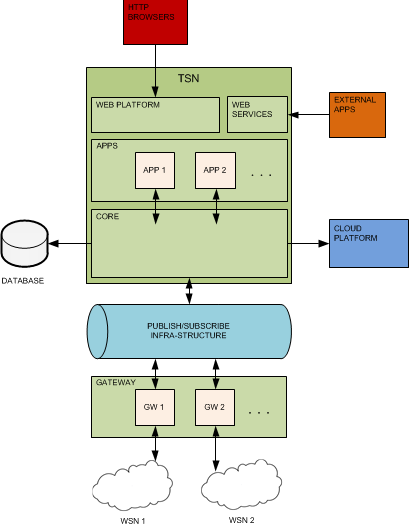
\includegraphics[scale=0.5]{./images/37-ttsp-tsn_ng.png}
\end{center}
\caption{Tagus-SensorNet proposed architecture.}
\label{tsnng}
\end{figure}

The major contribution with this design is made by the publish/subscribe infra-structure which is able to support multiple communication flows through message label multiplexing, this offers extremely flexibility on the way applications interact with different WSNs and eventually nodes. Applications publish messages to specific WSN islands and nodes. On the other end gateways subscribe to those messages and convert the message to the specific network protocol being executed at that WSN island and vice-versa.\\
This new architecture clearly enables a new paradigm of WSN application development flexibility and interaction. Other components were thought to be added in a future stage, such as interface with a cloud computing platform, export a Web Services API to allow other ways of interfacing with Tagus-SensorNet and GUI related interfaces. With this said, Tagus-SensorNet architecture changes ease application development and interaction with the WSN, which eventually facilitated TTSP development and evaluation.\\

A global overview of f TTSP implementation considerations as also other related work was given throughout this chapter. It is worth to mention that TTSP’s reference implementation has been freely contributed to TinyOS contributions repository under the GEMS group directory.
\cleardoublepage

\chapter{TTSP Test and Evaluation}

%-----------------------------------------------------------
% keywords: Test-bed, Tests
%-----------------------------------------------------------
With the purpose of validating the proposed architecture, TTSP was deployed in a WSN test-bed and was subject to a series of test scenarios. These tests intend to evaluate the time synchronization in scenarios ranging from a single node to multiples nodes, from a single-hop network to a multi-hop network, from high precision requirements to much lower precision requirements. Since these tests were designed solely to show how TTSP's synchronization is effective and its features operate, in a qualitative manner, each test was run only once. Being this the case, the obtained results may only be used as a comparison between each test and to validate the effectiveness of the given functionality.\\
%-----------------------------------------------------------
% keywords: Tagus-SensorNet
%-----------------------------------------------------------
Regarding the test-bed, a WSN test-bed, Tagus-SensorNet \cite{conf/icccn/PedrosaMRN08}, allows the unique opportunity to test TTSP in a real deployment scenario, allowing it to experience the intrinsic constraints of a WSN. That is, in Tagus-SensorNet sensor nodes are faced with limited energy resources, communications that can easily be interfered and sensor nodes that can suddenly die or start functioning incorrectly.

\section{Test-bed and Test Scenarios}

\subsection{Tagus-SensorNet}
%-----------------------------------------------------------
% keywords: Tagus-SensorNet
%-----------------------------------------------------------
Tagus-SensorNet sensor nodes, as can be seen in Figure \ref{tsn}, are well dispersed in Taguspark main building.\\

\begin{figure}[!htb]
\begin{center}
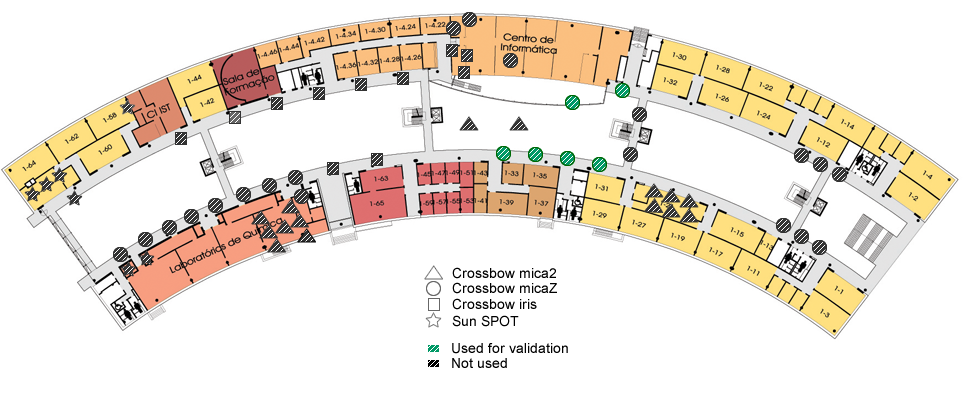
\includegraphics[scale=0.4]{./images/04-tsn-topology.png}
\end{center}
\caption{Tagus-SensorNet current deployment topology.}
\label{tsn}
\end{figure}
%-----------------------------------------------------------
% keywords: 
%-----------------------------------------------------------
The current topology, allows the creation of regions that currently cannot be interconnected, whether it be the physical distance or the heterogeneity of the communication stack, mainly found with the Sun SPOTs and the  Mica family sensor nodes (both Mica2 and MicaZ). Currently, these two family of sensor nodes do not communicate between themselves, although they both have a IEEE 802.14.15 capable radio. The Sun SPOTs run a Java VM while the Mica family sensor nodes run TinyOS.\\
%-----------------------------------------------------------
% keywords: 
%-----------------------------------------------------------
The radio communications that work on the 868/916 MHz and mainly in 2,4 GHz band, face possible interference of other radio technologies that operate on the same band, like IEEE 802.11. This imposes serious communication constraints. But nonetheless, short or long periods of interference are indeed a real
constraint of any WSN.\\
%-----------------------------------------------------------
% keywords: 
%-----------------------------------------------------------
The Mica family sensor nodes are powered by two AAA batteries which also impose serious network lifetime constraints. A sensor node may suddenly die once it's batteries are depleted or stop functioning correctly once the available voltage is lower than the necessary to keep micro-controller, the radio or any other hardware component running correctly.\\
As previously stated, all these constraints, give a unique opportunity for TTSP to be validated correctly, since the real requirements of a WSN are present on this testbed.


\subsection{Test Scenario}
%-----------------------------------------------------------
% keywords: Test Scenario
%-----------------------------------------------------------
The test scenario chosen for this purpose is described in Figure \ref{scenario6}. In this scenario, there are a total of five synchronizing nodes, of which, one node will be declared as the root node, four are to be synchronized with that root node at a given moment in time. One additional node is used as a base-station for continuously collecting the selected metrics from the synchronized nodes and the root node. 

\begin{figure}[!htb]
\begin{center}
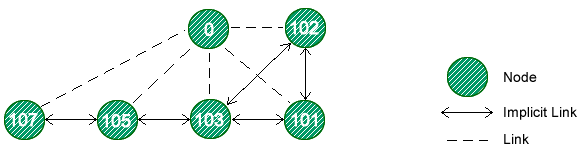
\includegraphics[scale=0.4]{./images/19-ttsp-test_topology.png}
\end{center}
\caption{Six nodes scenario with multi-hop synchronization.}
\label{scenario6}
\end{figure}

Although, most of the used nodes are in the radio coverage of each other, there was the need for a slightly different network topology that could best describe all the physical network topologies that are currently used by other applications in Tagus-SensorNet. For this reason, implicit links were statically configured in each node, which forced the desired logic topology as shown in the previous figure.

\section{Test Application and Methodology}
%-----------------------------------------------------------
% keywords: Test Application
%-----------------------------------------------------------
In order to produce meaningful results from the test-bed, a special test application was developed, which made use of TTSP libraries. This test application acted as an application client by declaring its time precision requirements to TTSP. Every node programmed with this test application was queried by the base-station in order to retrieve the current root node identification and its logical clock time. These values were periodically collected by the base-station, thus it was possible to periodically calculate the time precision error for every node that was synchronized with a root node.

\section{Test Results}
%-----------------------------------------------------------
% keywords: Test Results
%-----------------------------------------------------------
In this section, the processed test results will be presented and briefly discussed. The following indicators have been used across multiple tests:
\begin{itemize}
\item \textit{Precision Error}:  This value, as the name suggests, indicates the current time precision error achieved by a node when synchronized with the root node, measured in time units. This error is obtained from the difference between the local clock of the root node and the logical clock of the synchronizing node, and it is only relevant once this node declared itself synchronized with the root.
\item \textit{Synchronization Period}: This value indicates the current synchronization period being advertised by the root node to the synchronizing nodes. As explained in the previous chapter, the values that this indicator reports are deeply influenced by the current time precision error achieved with the synchronizing nodes.
\end{itemize}

\clearpage

\subsection{Single-hop/-node Synchronization With High Precision Requirements}
%-----------------------------------------------------------
% keywords: 
%-----------------------------------------------------------
A single-hop with only one node to synchronize with the root node is the basic scenario where TTSP can be used. This scenario was chosen in order to evaluate the efficiency and effectiveness of the TTSP's response which is directly influenced by the time precision error monitored from its synchronizing nodes, thus the number of synchronizing nodes is relevant for the evaluation of TTSP. For this first scenario a high precision requirement of a maximum time precision error of 10 ms was chosen. The results of this scenario can be found in Figure \ref{10ms2nodes}.

\begin{figure}[!htb]
\begin{center}
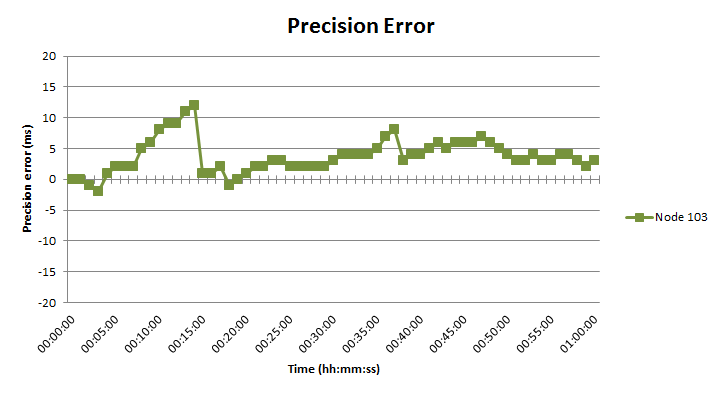
\includegraphics[scale=0.4]{./images/09-ttsp-10ms2nodes-error.png}
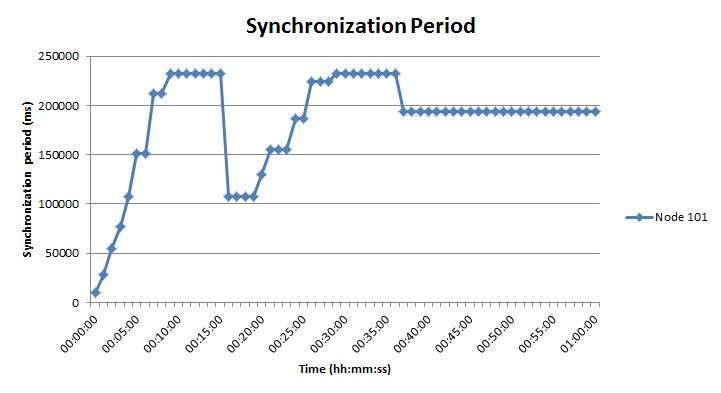
\includegraphics[scale=0.4]{./images/10-ttsp-10ms2nodes-period.png}
\end{center}
\caption{Single-hop/-node synchronization results with a precision error requirement of 10 ms.}
\label{10ms2nodes}
\end{figure}

The results indicate, that for a single-hop synchronization of a single node, the synchronization period converges to an approximated value of 194 seconds while ensuring that the time precision error is below the required value.

\subsection{Single-hop/-node Synchronization With Low Precision Requirements}
%-----------------------------------------------------------
% keywords:
%-----------------------------------------------------------
This scenario resembles almost everything with the previous one, except that the requested maximum time precision error is higher, thus a lower precision requirement which will also significantly influence the efficiency and effectiveness of TTSP's response. For the previous scenario of a single node a lower precision requirement of only 50 ms was required to TTSP. The obtained results are shown in Figure \ref{50ms2nodes}.

\begin{figure}[!htb]
\begin{center}
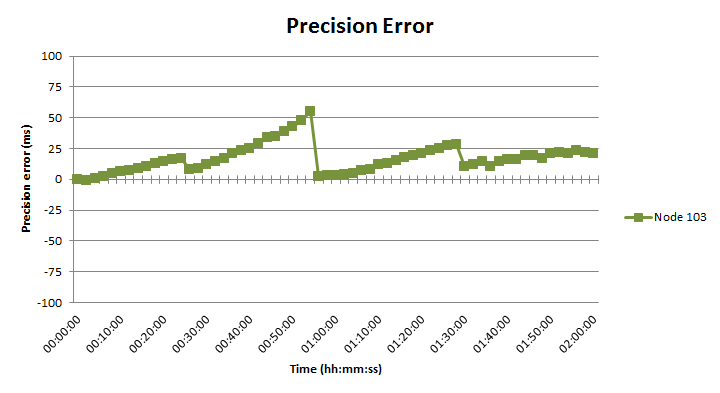
\includegraphics[scale=0.4]{./images/20-ttsp-50ms2nodes-error.png}
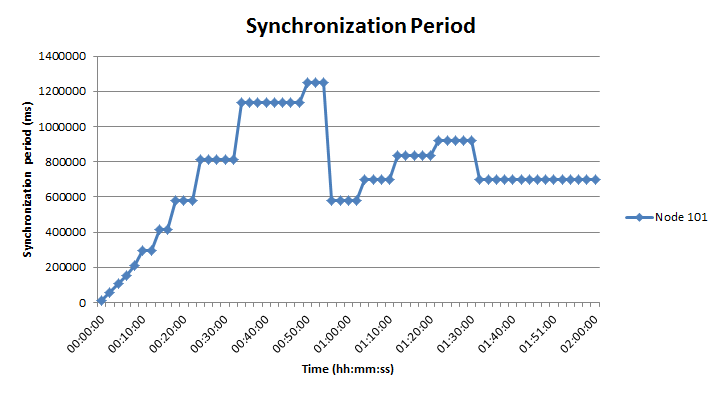
\includegraphics[scale=0.4]{./images/21-ttsp-50ms2nodes-period.png}
\end{center}
\caption{Single-hop/-node synchronization results with a error precision requirement of 50 ms.}
\label{50ms2nodes}
\end{figure}

The results show that for a time precision error lower than 50 ms, the synchronization period converges to an approximated value of 11 minutes and 37 seconds, which is entirely justified by the more relaxed precision requirements. One also needs to take into consideration the increased amount of time needed to converge to a synchronization period when compared with the results of the past scenario.

\subsection{Multi-hop/node Synchronization With High Precision Requirements}
%-----------------------------------------------------------
% keywords: multi-hop/node synchronization with high precision requirements
%-----------------------------------------------------------
In this scenario, multiple nodes are used with multi-hop being used by some of these in order for synchronization to be realized. This scenario is described in Figure \ref{scenario6}. For this scenario, it was requested from TTSP that the maximum precision error did not exceed the 10 ms. The obtained results in Figure \ref{10ms6nodes}.

\begin{figure}[!htb]
\begin{center}
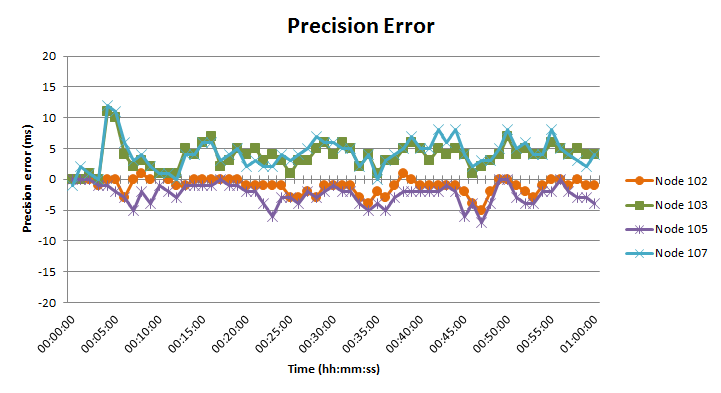
\includegraphics[scale=0.4]{./images/11-ttsp-10ms6nodes-error.png}
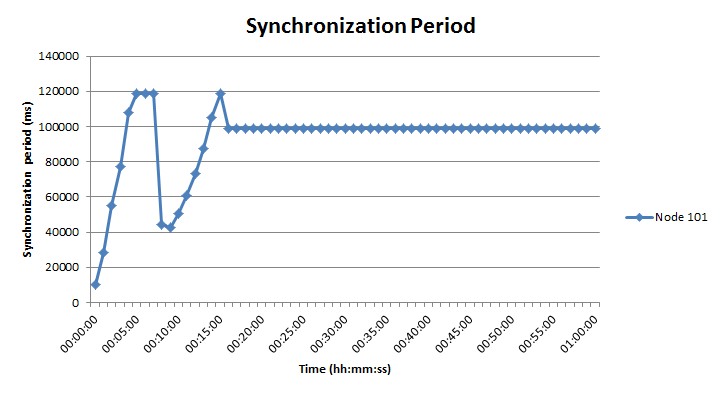
\includegraphics[scale=0.4]{./images/12-ttsp-10ms6nodes-period.png}
\end{center}
\caption{Time precision error with a precision request of 10 ms and using 6 nodes.}
\label{10ms6nodes}
\end{figure}

The results clearly show that for an increased number of synchronizing nodes, the synchronization period converges much faster, almost twice as fast when synchronizing only one node as shown in the first experiment results in Figure \ref{10ms2nodes} with the same time precision requirements. This is justified by the increased number of nodes, which allow for a faster synchronization period convergence, since multiple feedbacks are used to actuate on the synchronization period. Even though the root node filters neighbours feedback by the sequence number of the synchronization round, it also takes into account the total number of acceptable and unacceptable feedback received to adjust the synchronization period.
This awareness allows TTSP to converge the synchronization period faster. This fast convergence is clearly justified by the increased number of synchronizing nodes. Although, a fast convergence of the synchronization period was observed, the final achieved synchronization period was almost half as what was achieved with only one node. This can also be justified by the number of synchronizing nodes, more specifically the probability of existence of synchronizing nodes with clock drifts completely different than the root node, which will result in higher absolute precision errors, thus forcing a lower synchronization period for the network-wide synchronization.

\clearpage

\subsection{Multi-hop/-node Synchronization With Low Precision Requirements}
%-----------------------------------------------------------
% keywords: multi-hop/node synchronization with low precision requirements
%-----------------------------------------------------------
For this experiment, the previous scenario was used, the only changed parameter as like the experiment with the single-node, was the maximum time precision error allowed in the network. Thus, the maximum tolerable precision error was increased to 50 ms. The obtained results can be seen in Figure \ref{50ms6nodes}.

\begin{figure}[!htb]
\begin{center}
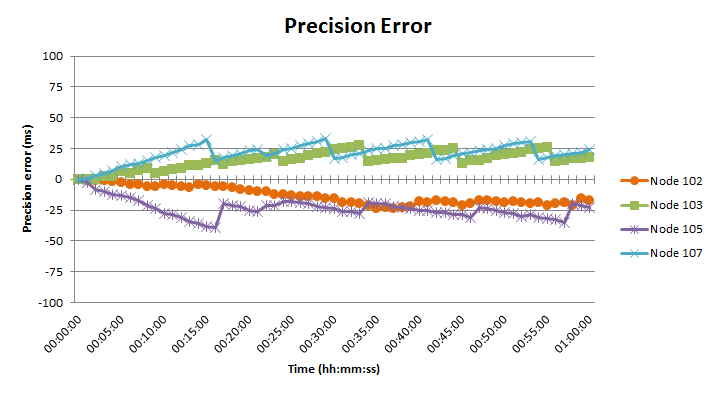
\includegraphics[scale=0.4]{./images/23-ttsp-50ms6nodes-error.png}
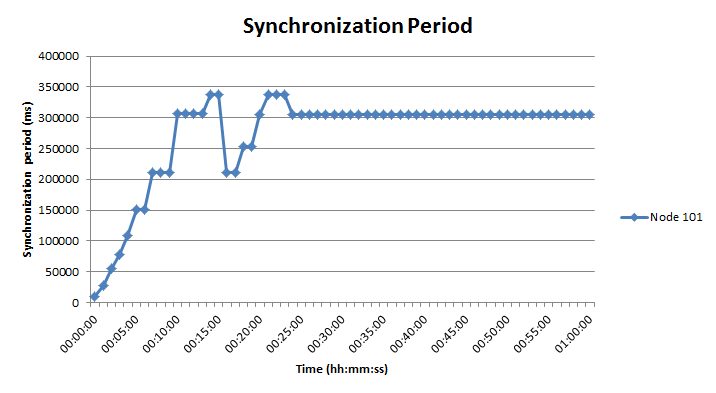
\includegraphics[scale=0.4]{./images/22-ttsp-50ms6nodes-period.png}
\end{center}
\caption{Time precision error with a precision request of 50 ms and using 6 nodes.}
\label{50ms6nodes}
\end{figure}

It is possible to conclude from these results, that the relaxation of the requirements tend to have the same effect as in the case of a single node, that is, a slower synchronization convergence but a higher synchronization period. One can extend this observation, by stating that the synchronization period converged at 24 minutes since the beginning of this experiment, eight more minutes than the needed in the previous experiment with a requirement of a time precision error below of 10 ms, showing that the difference is not that higher as with the experiment with the single-node.

\clearpage

\subsection{Fast Synchronization Mechanism}
%-----------------------------------------------------------
% keywords: fast synchronization mechanism
%-----------------------------------------------------------
The objective with this experiment is to assess the fast synchronization mechanism that is triggered when for example a node joins the network for a first time after the synchronization period has already converged or the re-election mechanism has been triggered and the information of the new root is being propagated throughout the network. In this typical situation the new node will have to collect four synchronization points from a root node or a neighbouring node. Without the use of this mechanism, the new node would have to wait for four times the current synchronization period in order to get synchronized with the root node. The fast mechanism basically detects new nodes and triggers a consecutive broadcast of four samples in order for the new node to get quickly synchronized with the root node. In Figure \ref{fastsync} it is possible to verify the obtained results with the use of this mechanism, it is important to detail that the new node (node 107) was turned on at exactly 40 minutes since the beginning of the test.

\begin{figure}[!htb]
\begin{center}
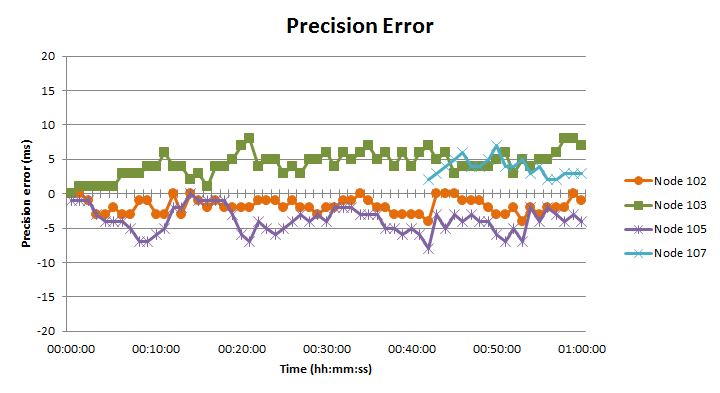
\includegraphics[scale=0.4]{./images/15-ttsp-10ms6nodes-fastsync-error.png}
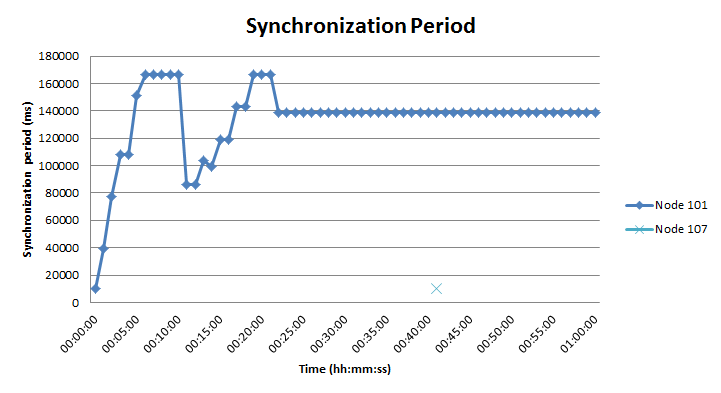
\includegraphics[scale=0.4]{./images/16-ttsp-10ms6nodes-fastsync-period.png}
\end{center}
\caption{Fast synchronization mechanism.}
\label{fastsync}
\end{figure}

Regarding this case, after the new node was turned on, and past the time duration of three times the initial synchronization period without hearing a synchronization broadcast, it declares itself root, in this case after 30 seconds, since the default initial synchronization period was set to 10 seconds. It could happen that the new node could hear a synchronization broadcast from one of its neighbours, which did not happened in this specific case. In those situations however, the new node would have discard the synchronization point by looking at the synchronization period which is clearly different from the initial synchronization period. Once the new node elects himself, he starts to broadcast its local clock with a period of 10 seconds. The first broadcast is heard by its neighbouring nodes which are already synchronized with root node with an identification lower than the new node. This triggers the fast synchronization mechanism in the neighbouring nodes, which leads the new node to be aware of the actual root node and became synchronized with it. 

\clearpage

\subsection{Re-election Mechanism}
%-----------------------------------------------------------
% keywords: re-election mechanism
%-----------------------------------------------------------
In this experiment, the objective is to assess the re-election mechanism which must be executed once the current root node ceases to broadcast its local clock. The used scenario is the same as the one used with the multiple nodes and existence of multi-hop synchronization. The experiment is composed of a initial period where all synchronizing nodes will eventually synchronize with an elected root node, and consequently that root node will be remotely turned off, ceasing to broadcast its local clock. The remaining nodes, must continue to be synchronized among themselves, for that, the re-elections mechanism will be triggered and a new root node elected. The results of this experiment can be seen in Figure \ref{reelection}.

\begin{figure}[!htb]
\begin{center}
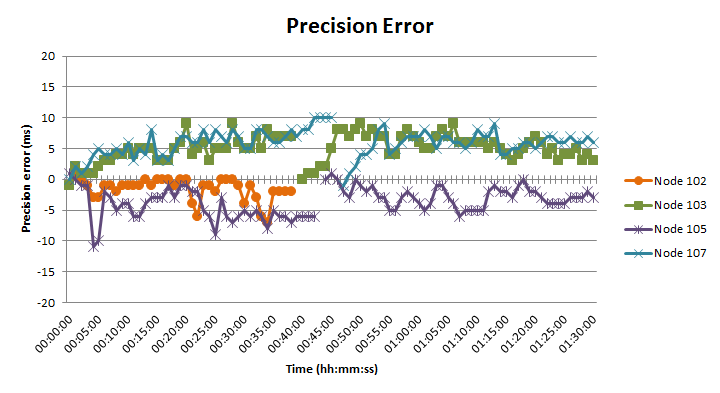
\includegraphics[scale=0.4]{./images/13-ttsp-10ms6nodes-reelection-error.png}
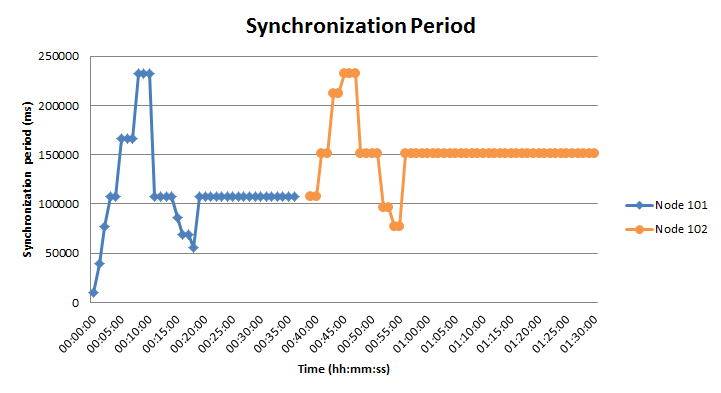
\includegraphics[scale=0.4]{./images/14-ttsp-10ms6nodes-reelection-period.png}
\end{center}
\caption{Re-election mechanism.}
\label{reelection}
\end{figure}

The results are clear enough to tell that the new root node is elected, the remaining node with the lower identification. This process is triggered on each node after a root silence of three times the current synchronization period. In this case, 312 seconds after the first root node broadcasted its last local clock. After the re-election process is triggered,  the recent elected node continues with the same synchronization period than its predecessor, but becomes aware of the current low absolute precision error gathered from the synchronizing nodes and adaptively adjusts the synchronization period to a best suitable one.

\clearpage

\subsection{Multi-hop/-node Synchronization with High Requirements Extended Duration}
%-----------------------------------------------------------
% keywords: 
%-----------------------------------------------------------
This experiments objective was different from the previous ones. The sole purpose of this experiment is to assess the effectiveness of TTSP synchronization over a longer period. This experiment was necessary due to the stringent need of keeping the maximum precision error lower than the requested and keep the synchronization period stable over a longer period. A twenty-four hour experiment of TTSP on Tagus-SensorNet is acceptable for this objective and the obtained results can be seen in Figure \ref{24h}.

\begin{figure}[!htb]
\begin{center}
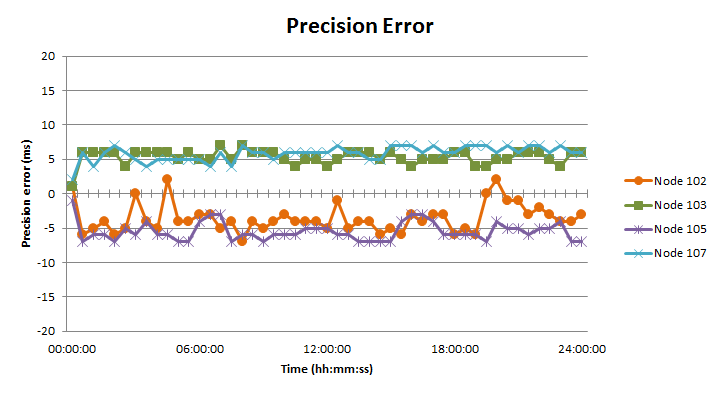
\includegraphics[scale=0.4]{./images/17-ttsp-10ms5nodes-error.png}
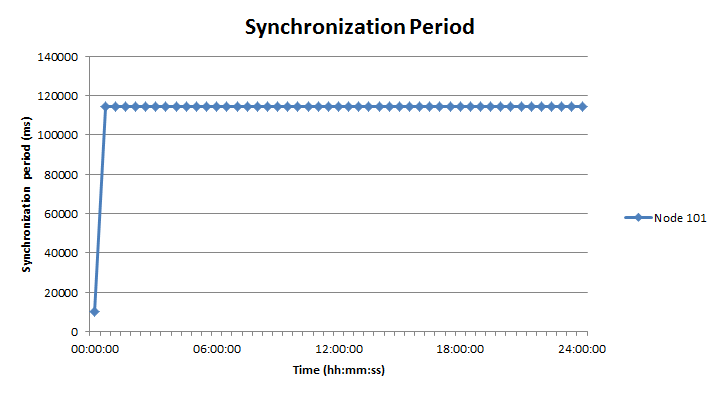
\includegraphics[scale=0.4]{./images/18-ttsp-10ms5nodes-period.png}
\end{center}
\caption{Time precision error with a precision request of 10 ms and using 5 nodes.}
\label{24h}
\end{figure}

As predicted, without any changes involving the root node, the time precision error on all nodes in the network keeps below the maximum allowed threshold and the synchronization period keeps unchanged. One can conclude, that the requirements were fulfilled during this twenty-four hour period, and the time synchronization protocol operated stable under normal circumstances that Tagus-SensorNet is daily subject to. The interference from closely wireless networks such as the campus 802.11 infrastructure network (which covers the whole main building) did not significantly influenced TTSPs effectiveness as all nodes kept synchronized with a precision error lower than the requested throughout the twenty-four hour period.
\cleardoublepage

\chapter{Conclusions}

%-----------------------------------------------------------
% keywords: Time synchronization in WSN, classic protocols
%-----------------------------------------------------------
The need for time synchronization in WSNs is critical for data consistency, MAC protocols and ultimately extending the network lifetime with coordinated sleeping and wake up cycles. Classic time synchronization protocols found on wired and common wireless networks, do not fill the necessary requirements for being deployed on a WSN.\\

%-----------------------------------------------------------
% keywords: Available time synchronization protocols for WSNs
%-----------------------------------------------------------
However, there has been effort on developing time synchronization protocols that do try to meet the requirements of time synchronization on WSNs. These protocols can be broadly classified by their approaches to pair-wise and network-wide synchronization. Common approaches found for pair-wise synchronization are implemented by a scheme of Sender-to-receiver or a Receiver-to-receiver. While for network-wide synchronization common approaches used are a Master-slave or a Peer-to-peer scheme. These classifications broadly classify a time synchronization protocol, although there are many other aspects to take into account. One common metric of performance used by many authors to evaluate their own protocol, its the time precision error obtained. It is evident that, lower time precision error obtained, more time precision is given to the applications operating on the WSN. But most of the times we might be spending a lot of effort on delivering a time precision that is not needed by the application itself. This effort is intrinsically linked with the usage of the scarce resources that are available on the WSN. A lifetime of a WSN weighs heavily with the energy resources that are available to it. The problem of wasting valuable amounts of these resources while seeking a time precision that is not required by the application, is critical and has not been clearly addressed by the protocols found on this related work.\\

%-----------------------------------------------------------
% keywords: TTSP architecture
%-----------------------------------------------------------
TTSP provides the capability of fulfilling the synchronization time precision requirements declared by its clients, whether they be the user application running on the nodes or the MAC-layer protocol residing in the operating system of the nodes. The requirements are stated through specific interfaces, which indicate TTSP to keep the synchronization time precision errors below that threshold. Knowing the requested maximum time precision error allowed, TTSP adjusts its synchronization period so that it can minimize the use of its limited resources while keeping every node synchronized with their time precision errors below the requested threshold. TTSP uses a sender-to-receiver scheme for pair-wise synchronization and a master-slave scheme for network-wide synchronization. Several commonly synchronization techniques from these schemes are used. These involve synchronization through message exchange, MAC-layer time-stamping, synchronization in rounds, skew compensation, controlled flooding of broadcasted messages and a master re-election mechanism. To assure that the time precision errors are acceptable within the network, the root node (to which every other node is being synchronized with) is constantly monitoring its synchronizing nodes through their synchronization broadcasts, or in case of a multi-hop, through a forwarded synchronization broadcast. Adjustments to the synchronization period, are taken from these feedback, typically acceptable time precision errors tend to allow a higher synchronization period, while unacceptable precision errors tend to force a decrease of the synchronization period. Thus, the root node adaptively adjusts the synchronization period solely based on the results of its past actions on the synchronization period.\\ 

%-----------------------------------------------------------
% keywords: TTSP implementation
%-----------------------------------------------------------
A reference implementation of TTSP was developed in TinyOS, which is the most popular and open-source operating system available at the moment. TinyOS provides an event-centric and modular architecture, which allowed TTSP implementation development to take benefits from both of these architecture approaches.\\

%-----------------------------------------------------------
% keywords: Evaluation
%-----------------------------------------------------------
Validation of TTSP was conducted in Tagus-SensorNet, a WSN test-bed, which served as a way of assessing TTSP complexity and to collect real-world performance data. The following are some of the most relevant data collected:
\begin{itemize}
\item Regarding the scalability issues when tested with only one and four synchronizing nodes, TTSP tends to converge to a synchronization period faster when more nodes are present in the network, this is clearly justified by the increased quantity of feedback returned from its adjustments. But the increased number of nodes also give room to nodes with completely different clock drift rates than the one from the root node, which in the end, leads to a lower synchronization period, thus a higher resource consumption.
\item A set of time precision requirements were tested, precisely a maximum precision error of 10 ms and 50 ms. Both requirements are fulfilled, although one can observe that for a lower requirement, in this case the 50 ms requirement, the synchronization period convergence seems to be slower than the higher one. This is justified by the intrinsic mechanism of an adaptive approach, in which an adjustment is made and future adjustments will solely depend on the outcome of the received feedback of that previous adjustment. In this particular case, requesting a lower requirement, will let TTSP reach long synchronization periods, which will result in longer feedbacks, thus a slower synchronization period convergence.
\item The fast synchronization mechanism in TTSP allows new arriving or just turned on nodes, to quickly synchronize with the root node after it has already converged to a synchronization period. This mechanism avoids unacceptable waiting times by allowing a new node to synchronize with the root node in less than a minute after it has been detected.
\item Finally, a long run test of TTSP was tested for twenty-four hours, in which the test-bed was subject to all kinds of radio interference which is common in Tagus-SensorNet. The results showed that TTSP guaranteed that the maximum precision error was not reached and that once the synchronization period converged it didn't suffer any changes. This clearly fulfils the objective of adaptively synchronizing Tagus-SensorNet while fulfilling specific time precision requirements.
\end{itemize}

%-----------------------------------------------------------
% keywords: Final conclusion
%-----------------------------------------------------------
The results obtained with TTSP in Tagus-SensorNet make it a valid approach to synchronize clocks in WSNs. By using TTSP for time synchronization in a WSN, it's possible to adapt the time synchronization period to fulfil the time precision requirements while seeking to minimize the resource consumption in the process. TTSP also avoids statically pre-configured synchronization periods which might end not being suitable if for any reason the network topologies changes or nodes get removed or added to the network. TTSP cleverly finds the adequate synchronization period for the requested maximum time precision error allowed in the network, thus avoiding network administrator parametrization. One can also conclude that by using TTSP, it will be possible to maximize the network lifetime, since the most power demanding component of a node, the radio used for message transmission and reception is less used when a better suitable (obtained with TTSP) synchronization period is used. Finally, TTSP accomplishes the initial proposed goals, that is to achieve a network-wide synchronization in a scalable fashion way with requested specific time precision requirements while making an efficient use of the available network resources.

\section{Future Work}

Regarding TTSP, there are some challenges and space for improvement in a future work. The following open issues are but some of the ones that come to mind for further development:
\begin{itemize}
\item TTSP uses a modular architecture, its underlying time synchronization logic can easily be switched as long as it still maintains and makes use of the same interface signatures. Thus, a suggestion would be to adopt other synchronization approach schemes, such as a Receiver-to-receiver scheme for pair-wise synchronization or a Peer-to-peer for network-wide synchronization.
\item Integrating techniques for secure time synchronization in TTSP could prove useful for resilient WSNs.
\item Executing a series of extensive tests in Tagus-Sensornet with different MAC protocols and different time precision requirements or maximum synchronization period.
\item TTSP can easily support node mobility by maintaining a set of samples for each root a node finds during its lifetime, thus allowing multi-root synchronization, this feature has not be tested extensively in Tagus-SensorNet, but should be done for future work, it would also aid in identifying current weaknesses (limitations such as memory size) and elaborate optimizations.
\end{itemize}
\cleardoublepage

\pdfbookmark[0]{Bibliography}{bib}
\bibliographystyle{IEEEtran}
\bibliography{bibliography}

%\appendix
%\pdfbookmark[1]{Appendix A}{appendix}
%\chapter{Synchronization period adjustment flowchart}

\begin{figure}[!htb]
\begin{center}
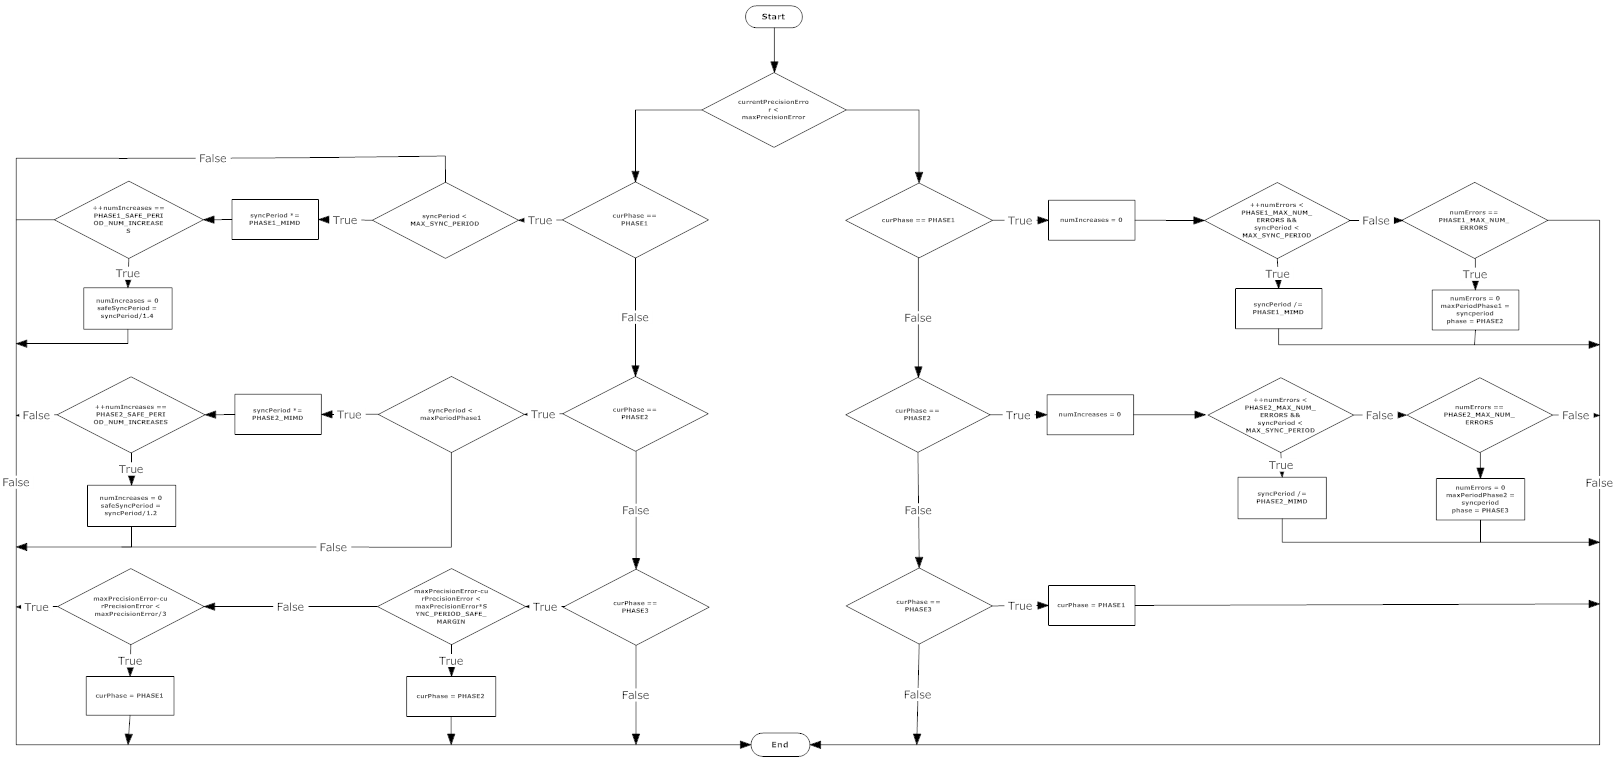
\includegraphics[scale=0.4,angle=90]{./images/26-ttsp-flowchart.png}
\end{center}
\caption{Detailed flowchart of the synchronization period adjustment algorithm.}
\label{flow}
\end{figure}

\cleardoublepage
\cleardoublepage
\end{document}
